\documentclass[12pt]{article}
\pagestyle{plain}
\pdfoutput=1
\usepackage{geometry}
\geometry{verbose,tmargin=1in,bmargin=1in,lmargin=1in,rmargin=1in}
\usepackage{lmodern}
\usepackage{amsmath}
\usepackage{amssymb}
\usepackage{amsthm}
\usepackage{color}
\usepackage[usenames,dvipsnames]{xcolor}
\usepackage{graphicx}
\usepackage{threeparttable}
%\usepackage{subcaption}
\usepackage{forest} 
\usepackage{soul}
\usepackage{subfig}
\usepackage{booktabs}
\usepackage{bigints}
\usepackage[countmax]{subfloat}
\usepackage{float}
\usepackage{rotfloat}
\usepackage{bm}
\usepackage{comment}
\usepackage{enumerate} 
\usepackage{setspace}
\usepackage{esint} 
\usepackage{pdflscape}
\usepackage{tikz}
\usetikzlibrary{snakes}
\usetikzlibrary{decorations.pathreplacing}
\usepackage{pdfpages}
\usepackage{enumitem}
\usepackage{diagbox}
\usepackage{lscape}
\usepackage{multirow}
\usepackage{ragged2e}
\usepackage{tabularx}
\usepackage{mathrsfs}
\usepackage{adjustbox}
\usepackage{mathtools}
\usepackage{placeins}
\usepackage{yhmath}

\usepackage[T1]{fontenc}


%\usepackage{subcaption}
\doublespacing
\usepackage[authoryear]{natbib}
\definecolor{MyDarkBlue}{rgb}{0,0.08,0.45}
\usepackage[unicode=true,pdfusetitle, bookmarks=true,bookmarksnumbered=false,bookmarksopen=false, breaklinks=false,pdfborder={0 0 1},backref=section,colorlinks=true, linkcolor = MyDarkBlue, citecolor = MyDarkBlue]{hyperref}
% \usepackage{breakurl}
\PassOptionsToPackage{normalem}{ulem}
\usepackage{ulem}
\makeatletter
\numberwithin{equation}{section}
\hypersetup{colorlinks=true, linkcolor=MyDarkBlue}
\usepackage[backgroundcolor = white, linecolor = red, bordercolor = red]{todonotes}
%\usepackage[backgroundcolor = white, linecolor = red, bordercolor = red, disable]{todonotes}
% TODO notes: simply uncomment the ,disable version if want to turn these off

\usepackage{scalerel,stackengine}
\stackMath
\newcommand\reallywidehat[1]{%
\savestack{\tmpbox}{\stretchto{%
  \scaleto{%
    \scalerel*[\widthof{\ensuremath{#1}}]{\kern-.6pt\bigwedge\kern-.6pt}%
    {\rule[-\textheight/2]{1ex}{\textheight}}%WIDTH-LIMITED BIG WEDGE
  }{\textheight}% 
}{0.5ex}}%
\stackon[1pt]{#1}{\tmpbox}%
}

\renewcommand*\thesubfigure{\arabic{subfigure}} 
\captionsetup[subfigure]{listofformat=subsimple}


\newtheorem{innercustomgeneric}{\customgenericname}
\providecommand{\customgenericname}{}
\newcommand{\newcustomtheorem}[2]{%
  \newenvironment{#1}[1]
  {%
   \renewcommand\customgenericname{#2}%
   \renewcommand\theinnercustomgeneric{##1}%
   \innercustomgeneric
  }
  {\endinnercustomgeneric}
}



\newcustomtheorem{claim}{{\bf \sc Claim}}
\newcustomtheorem{definition}{{\bf \sc Definition}}
\theoremstyle{theorem}\newcustomtheorem{theorem}{{\bf\sc Theorem}}
\newcustomtheorem{lemma}{{\bf\sc Lemma}}
\newcustomtheorem{example}{{\bf\sc Example}}
\newcustomtheorem{corollary}{{\bf\sc Corollary}}
\newcustomtheorem{conjecture}{{\bf\sc Conjecture}}
\theoremstyle{definition}\newcustomtheorem{assumption}{{\bf\sc Assumption}}
\theoremstyle{theorem} \newcustomtheorem{proposition}{{\bf\sc Proposition}}
\newcustomtheorem{rem}{{\bf \sc Remark}}
\newcustomtheorem{alg}{{\bf\sc Algorithm}}



\DeclareMathOperator*{\plim}{plim}
\DeclareMathOperator*{\argmin}{argmin}
\DeclareMathOperator*{\argmax}{argmax}
\DeclareMathOperator*{\cvgto}{\stackrel{\mathrm{P}}{\longrightarrow}}
\DeclareMathOperator*{\wkto}{\rightsquigarrow}
\providecommand{\E}{\mathbb{E}}
\providecommand{\var}{\mathrm{var}}
\providecommand{\Bin}{\mathrm{Bin}}
\providecommand{\corr}{\mathrm{corr}}
\providecommand{\cov}{\mathrm{cov}}
\providecommand{\aut}{\mathrm{aut}}
\providecommand{\Skew}{\mathrm{Skew}}
\providecommand{\Prob}{\mathrm{P}}
\providecommand{\thetahat}{\widehat{\theta}}
\providecommand{\gammahat}{\widehat{\gamma}}
\providecommand{\betahat}{\widehat{\beta}}
\providecommand{\phat}{\widehat{p}}
\providecommand{\Stil}{\widetilde{S}}
\renewcommand{\Pr}{\Prob}

\newcommand{\tH}{\text{H}}
\newcommand{\tL}{\text{L}}
\newcommand{\tM}{\text{M}}
\newcommand{\tU}{\text{U}}
\newcommand{\tw}{\text{w}}
\newcommand{\norm}[1]{\left\lVert#1\right\rVert}



\providecommand{\g}{{\bf g}}
\providecommand{\bfH}{{\bf H}}
\providecommand{\bfv}{{\bf v}}
\def\Re{\mathbb{R}}
\def\eproof{\hbox{\hskip3pt\vrule width4pt height8pt depth1.5pt}}
\renewenvironment{proof}[1][Proof]{\noindent\text{#1.} }{\ \rule{0.5em}{0.5em}}

\newenvironment{wideitemize}{\itemize\addtolength{\itemsep}{10pt}}{\enditemize}

\date{}

\newlength\mylen
\newcommand\bigbrace[2]{%
	\settowidth\mylen{$\displaystyle #1$}
	\underbrace{#1}_{\parbox{\mylen}{\scriptsize\Centering #2}}}


\title{Tracking Employment Changes in AI-Exposed Jobs}

\author{Bharat Chandar \footnote{Stanford University; \href{mailto:email}{\texttt{chandarb@stanford.edu.}} Thanks to Erik Bynjolfsson, Basil Halperin, Philip Trammell, Luca Vendraminelli, Tom Mitchell, and Ruyu Chen for helpful comments.}}

\date{\today}


\begin{document}

\maketitle

\begin{abstract}
	This paper examines labor market trends for occupations exposed to Generative AI using US Current Population Survey (CPS) data from the post-ChatGPT era (Q4 2022 - Q1 2025). Contrary to displacement fears, occupations most exposed to AI on average show no substantial difference in employment or earnings growth compared to the least exposed. However, this aggregate trend masks heterogeneity across occupations. Within the most exposed quartile, occupations with a higher share of college-educated workers, such as software development, have experienced robust employment growth, while those with a lower share, like customer service, have seen declines. The analysis also reveals a divergence between job posting data and realized employment, urging caution when inferring labor market trends from postings alone.
\end{abstract}

\setlength{\abovedisplayskip}{6pt}
\setlength{\belowdisplayskip}{6pt}

\section{Introduction}

The period following the public release of ChatGPT in November 2022 has seen burgeoning research attempting to capture the labor market and productivity effects of generative AI, spurred by fear of potential widespread job displacement. This paper provides a timely empirical analysis of this evolving landscape by leveraging U.S. Current Population Survey (CPS) data through Q1 2025. Using the GPT-4-based occupational exposure metrics from \citet{eloundou_gpts_2024}, I examine realized employment and earnings trends to measure whether, and how, disruption from new AI technologies is appearing in the U.S. workforce.

The central finding is that the most AI-exposed set of occupations has not experienced a declining share of employment, though among this group there is considerable heterogeneity in labor market trends. Software occupations, which are estimated to have high exposure to generative AI, show employment gains as of the first quarter of 2025. In contrast, customer service representatives, who also have high measured exposure, have experienced relative employment declines. More broadly, within the most exposed quartile, occupations with a higher share of college-educated workers have experienced faster employment growth over the prior four years compared to occupations with a lower college share. The results suggest a nuanced view of how measured AI or automation exposure affect employment, with worker characteristics such as education potentially influencing displacement from new technologies. While the results do not identify a causal impact of AI on labor market outcomes, they clarify facts about the state of the US labor market and suggest avenues for further study on how AI impacts workers.\footnote{Another way to interpret the results is that current AI exposure and automation measures may do a poor job of predicting the true labor market impacts of AI, at least in the relatively short time period considered here. This contrasts with findings in prior seminal work such as \citet{autor_skill_2003} that showed that task exposure to computerization strongly predicted changes in relative labor demand.}

Given growing concern over AI's impact on early-career roles, I also examine trends for entry-level workers \citep{thompson_something_2025,raman_opinion_2025,allen_behind_2025}. Employment for entry-level workers is volatile and cyclical, making it difficult to discern trends. With more time and larger surveys it may become apparent whether there are sustained changes in labor market outcomes for entry-level workers, but so far evidence from the CPS is inconclusive. 

A further contribution of this paper is to highlight the divergence between employment and job postings. While Indeed job postings for software development show a decline from a peak in early 2022, CPS employment data indicate stable or even increasing employment through Q1 2025. The disconnect between job postings and employment also tracks with a relatively stable US national unemployment rate and labor force participation rate over the same period. These findings urge caution in interpreting labor market trends from job postings alone.

Because the CPS is released monthly and is publicly accessible, the method in this paper can be used to track changes in occupational employment on an ongoing and transparent basis. While the CPS's sample size limits statistical power for granular groups like entry-level workers, its strength lies in providing a consistent, high-frequency view of the entire U.S. labor market. This paper thus clarifies the current state of facts and provides a foundation for future work using larger-scale administrative or internal Census data to further probe the mechanisms behind these divergent outcomes.\footnote{All code is posted online at \url{https://github.com/chandarb/CPS_tracker}.} 

\section{Related Literature}

This paper engages with three active areas of research on the labor market effects of artificial intelligence. First, it builds on literature that measures AI's \emph{potential} exposure. A series of influential papers established methodologies for estimating which occupations were susceptible to automation \citep{frey_future_2017,brynjolfsson_what_2018,felten_method_2018, felten_occupational_2019,webb_impact_2019,felten_occupational_2021}. More recently, work such as \citet{eloundou_gpts_2024, felten_how_2023, gmyrek_generative_2023}, and \citet{gmyrek_generative_2025} adapted this approach for Generative AI, forming the basis for exposure metrics used in this analysis. While these studies identify potential disruption, this paper's contribution is to use broad, representative U.S. survey data (the CPS) to provide one of the earliest empirical snapshots of realized employment changes in the post-ChatGPT era. This complements studies that find significant effects but in more specific settings, such as on online freelance platforms \citep{hui_short-term_2023} or within individual firms \citep{brynjolfsson_generative_2025,dillon2025early}.\footnote{See also \citet{noy_experimental_2023,peng_impact_2023,dellacqua_navigating_2023}.}

Second, this paper contributes to the growing body of work using economy-wide data to measure AI's impact. Recent findings have been varied. \citet{humlum_large_2025} use Danish administrative data to find minimal effects on earnings or hours worked, while \citet{jiang_ai_2025} find AI exposure is correlated with longer work hours in the U.S.\footnote{See also \citet{acemoglu_artificial_2022,bonney_impact_2024,bick_rapid_2024,hartley_labor_2024, frank_ai_2025,chen_displacement_2025,hampole_artificial_2025}. The Federal Reserve Bank of New York tracks employment by college major using the American Community Survey (ACS), as documented in \citet{abel_underemployment_2017}. While the ACS has rich sociodemographic and economic information, it is released annually and with a time lag. As of Q2 2025 the latest ACS data is from 2023, in the initial year of LLM adoption.} This paper adds additional color to this growing set of findings. In line with \citet{humlum_large_2025}, I find little evidence of an aggregate decline in employment for exposed occupations. However, in contrast to their work, I find heterogeneity in employment trends across exposed occupations, with these differences correlated with features such as education. The divergent paths of software developers and customer service representatives, for example, suggest nuance in predictions of labor market changes for exposed workers.\footnote{Another closely related paper is \citet{deming_technological_2025}, which combines data from the decennial Census, Amercain Community Survey, and CPS to track labor market changes over 120 years. This paper complements their work by directly associating employment changes with measures of AI exposure and by tracking labor market trends specifically over the post-ChatGPT time period. }

Finally, this work highlights an important methodological issue: the divergence between job postings and employment data. Recent studies have used job postings to measure shifts in labor demand from AI (e.g., \citet{acemoglu_artificial_2022,hampole_artificial_2025}). This paper shows that for key occupations, these two data sources tell different stories. The decline in software developer job postings since 2022, for instance, contrasts sharply with their stable-to-growing employment in the CPS. This finding serves as an important empirical caution in interpreting job posting trends as reflective of employment or earnings. The CPS data used here provides a transparent and timely alternative for tracking realized outcomes as they unfold for a representative sample of the U.S. population.


\section{Methods and Data Collection} 

\subsection{Data on AI Exposure}

I use the occupation-level AI exposure estimates from \citet{eloundou_gpts_2024}. The authors estimate AI exposure based on O*NET task and detailed work activity (DWA) descriptions. I use their exposure measures that leverage GPT-4 to classify all tasks and DWAs based on the whether using an LLM reduces the time it takes to complete the task by at least 50\%. I aggregate from tasks to occupations by equally weighting exposure across tasks within an occupation. 

\citet{eloundou_gpts_2024} report a variety of different exposure measures based on this approachs. Each measure varies assumed capabilities of LLMs, namely whether they can reduce the time to complete a task on their own or in conjunction with additional software. I focus on their GPT-4-based $\beta$ measure for most of the analysis, though I show robustness to alternative measures for certain results.  

\subsection{Data on Employment and Earnings}

Employment and earnings data comes from the Current Population Survey (CPS). I use the CPS monthly employment file, focusing on the period from Q4 2022 onwards. This coincides with the period after the release of ChatGPT, which rapidly accelerated the use of LLMs in common practice. 

The CPS samples about 60,000 households each month. It reports employment status for each member of the household along with their Census occupation code, education, and other demographic variables. This information in the CPS is used to compute the official US Bureau of Labor Statistics (BLS) national unemployment rate. 

I use the merged outgoing rotation group (MORG) data to collect weekly earnings information. The MORG data is a subsample of the CPS that includes earnings data for workers in months four and eight of the sample.\footnote{Workers are surveyed for four months consecutively and then rotated out of the sample for four months before being rotated back in for another four months. } Because the MORG data is a subset of the basic monthly CPS it has a smaller sample size. The MORG data underwent changes in topcoding conventions over the sample period. I manually topcode nominal weekly earnings at \$2884.61 per week to maintain consistency over time. I also convert nominal weekly earnings to real weekly earnings using the CPI-U.

I merge the CPS data with the AI exposure estimates using the occupation code, using a crosswalk from the BLS to merge 2018 SOC codes to Census occupation codes. 

Computing employment trends by occupation can lead to noisy estimates due to small sample sizes. Further, the public monthly CPS file does not offer a straightfoward method to compute standard errors for employment estimates by occupation. To mitigate these issues, I compute the average monthly employment in each quarter and consider only analyses with at least 100 observations in each cell. 

\subsection{Summary Statistics}

Table \ref{tab:ai_exposure} shows the most and least AI-exposed occupations based on the GPT-4-based $\beta$ measure from \citet{eloundou_gpts_2024}. Professions involving translation, writing, and programming are among the most exposed, while occupations involving manual labor and construction are among the least exposed. 

\begin{table}[htbp]
	\centering
	\caption{Most and Least AI-Exposed Occupations. Exposure is defined using the GPT-4-based $\beta$ measure from \citet{eloundou_gpts_2024}. Occupations are 2018 Census occupation titles from the CPS merged via crosswalk to the 2018 SOC codes.}
	\begin{minipage}{0.48\textwidth}
		\centering
		\begin{tabular}{l}
			\hline
			\multicolumn{1}{c}{\textbf{Most Exposed Occupations}} \\
			\hline
			\\[-0.8em]
			Mathematicians \\[0.5em]
			Court reporters and simultaneous captioners \\[0.5em]
			Proofreaders and copy markers \\[0.5em]
			Correspondence clerks \\[0.5em]
			Computer programmers \\[0.5em]
			Web developers \\[0.5em]
			Database administrators and architects \\[0.5em]
			Telephone operators \\[0.5em]
			Interpreters and translators \\[0.5em]
			Writers and authors \\[0.5em]
			\hline
		\end{tabular}
	\end{minipage}
	\hfill
	\begin{minipage}{0.48\textwidth}
		\centering
		\begin{tabular}{l}
			\hline
			\multicolumn{1}{c}{\textbf{Least Exposed Occupations}} \\
			\hline
			\\[-0.8em]
			Athletes and sports competitors \\[0.5em]
			Packaging and filling machine operators \\[0.5em]
			Paper goods machine setters and operators \\[0.5em]
			Roustabouts, oil and gas \\[0.5em]
			Bus and truck mechanics \\[0.5em]
			Automotive glass installers and repairers \\[0.5em]
			Riggers \\[0.5em]
			Electrical power-line installers \\[0.5em]
			Excavating machine operators \\[0.5em]
			Rail-track maintenance operators \\[0.5em]
			\hline
		\end{tabular}
	\end{minipage}
	\label{tab:ai_exposure}
\end{table}

\section{Results}

\subsection{Labor Market Trends by AI Exposure}

Across all quartiles of AI exposure, there is little evidence of job loss or slower earnings growth for more exposed occupations since the release of ChatGPT. Figure \ref{fig:employment_trends} shows the employment and earnings trends for each quartile of AI exposure measured using the GPT-4-based $\beta$ metric. The plots shows the average employment and average real usual weekly earnings in each quarter for each quartile of AI exposure. Each series is normalized to 1 in Q4 2022, correponding to the time when ChatGPT was first released. The results suggest little if any evidence of relative employment declines in the most AI-exposed occupations since the release of ChatGPT. Real earnings have also grown at a similar rate. Figures \ref{fig:employment_trends_alpha} through \ref{fig:employment_trends_automation} show similar results using alternative measures of AI exposure. 

\begin{figure}[htbp]
	\centering
  \includegraphics[width=0.8\textwidth]{../figures/employment_share_by_gpt4_beta_quartile_2021q1.pdf}
  \includegraphics[width=0.8\textwidth]{../figures/real_earnings_by_gpt4_beta_quartile_2021q1.pdf}
	\caption{Employment and earnings trends by AI exposure. The top panel shows the share of employment by quartile of AI exposure, normalized to start at 1 in 2022 Q4. The AI exposure measure is the GPT-4-based $\beta$ measure from \citet{eloundou_gpts_2024}. Earnings are real usual weekly earnings, adjusted for inflation using the CPI-U and normalized to start at 1 in 2022 Q4.}
	\label{fig:employment_trends}
\end{figure}




\subsection{Software and Customer Service as Case Studies} 

Trends in the aggregate data mask the divergent patterns for key high-exposure occupations. This section presents two case studies—software developers and customer service representatives—that highlight this heterogeneity. Table \ref{tab:ai_exposure} shows that software development occupations have some of the highest estimated exposure to AI, consistent with LLMs being relatively proficient in writing computer code. Figure \ref{fig:employment_share_comparison_2021Q1} shows the employment trends for the Census occupation code corresponding to software developers. The results suggest an increase in employment in software development occupations since the release of ChatGPT. 

There are a variety of occupation codes that relate to computer programming, corresponding to codes 1005 through 1108. While software developers represent the largest share of employment in this group, one possibility is that employment gains for software developers come from reclassification of workers away from other coding occupations to software development.\footnote{See \citet{dam_more_2025} for a discussion of trends across different computer occupations.} Figure \ref{fig:employment_share_comparison_2021Q1} shows the employment and earnings trends for all computer occupations aggregated together. The results again suggest little evidence of a decline in employment or real earnings. 

The other series in Figure \ref{fig:employment_share_comparison_2021Q1} show employment and earnings trends for customer service representatives, another occupation in the top quartile of AI exposure. \citet{brynjolfsson_generative_2025} find that access to AI assistance increases worker productivity, as measured by issues resolved per hour, by 15\% on average for customer service representatives, with substantial heterogeneity across workers. Figure \ref{fig:employment_share_comparison_2021Q1} suggests that employment in customer service representatives has declined since the release of ChatGPT. 



\begin{figure}[htbp]
	\centering
  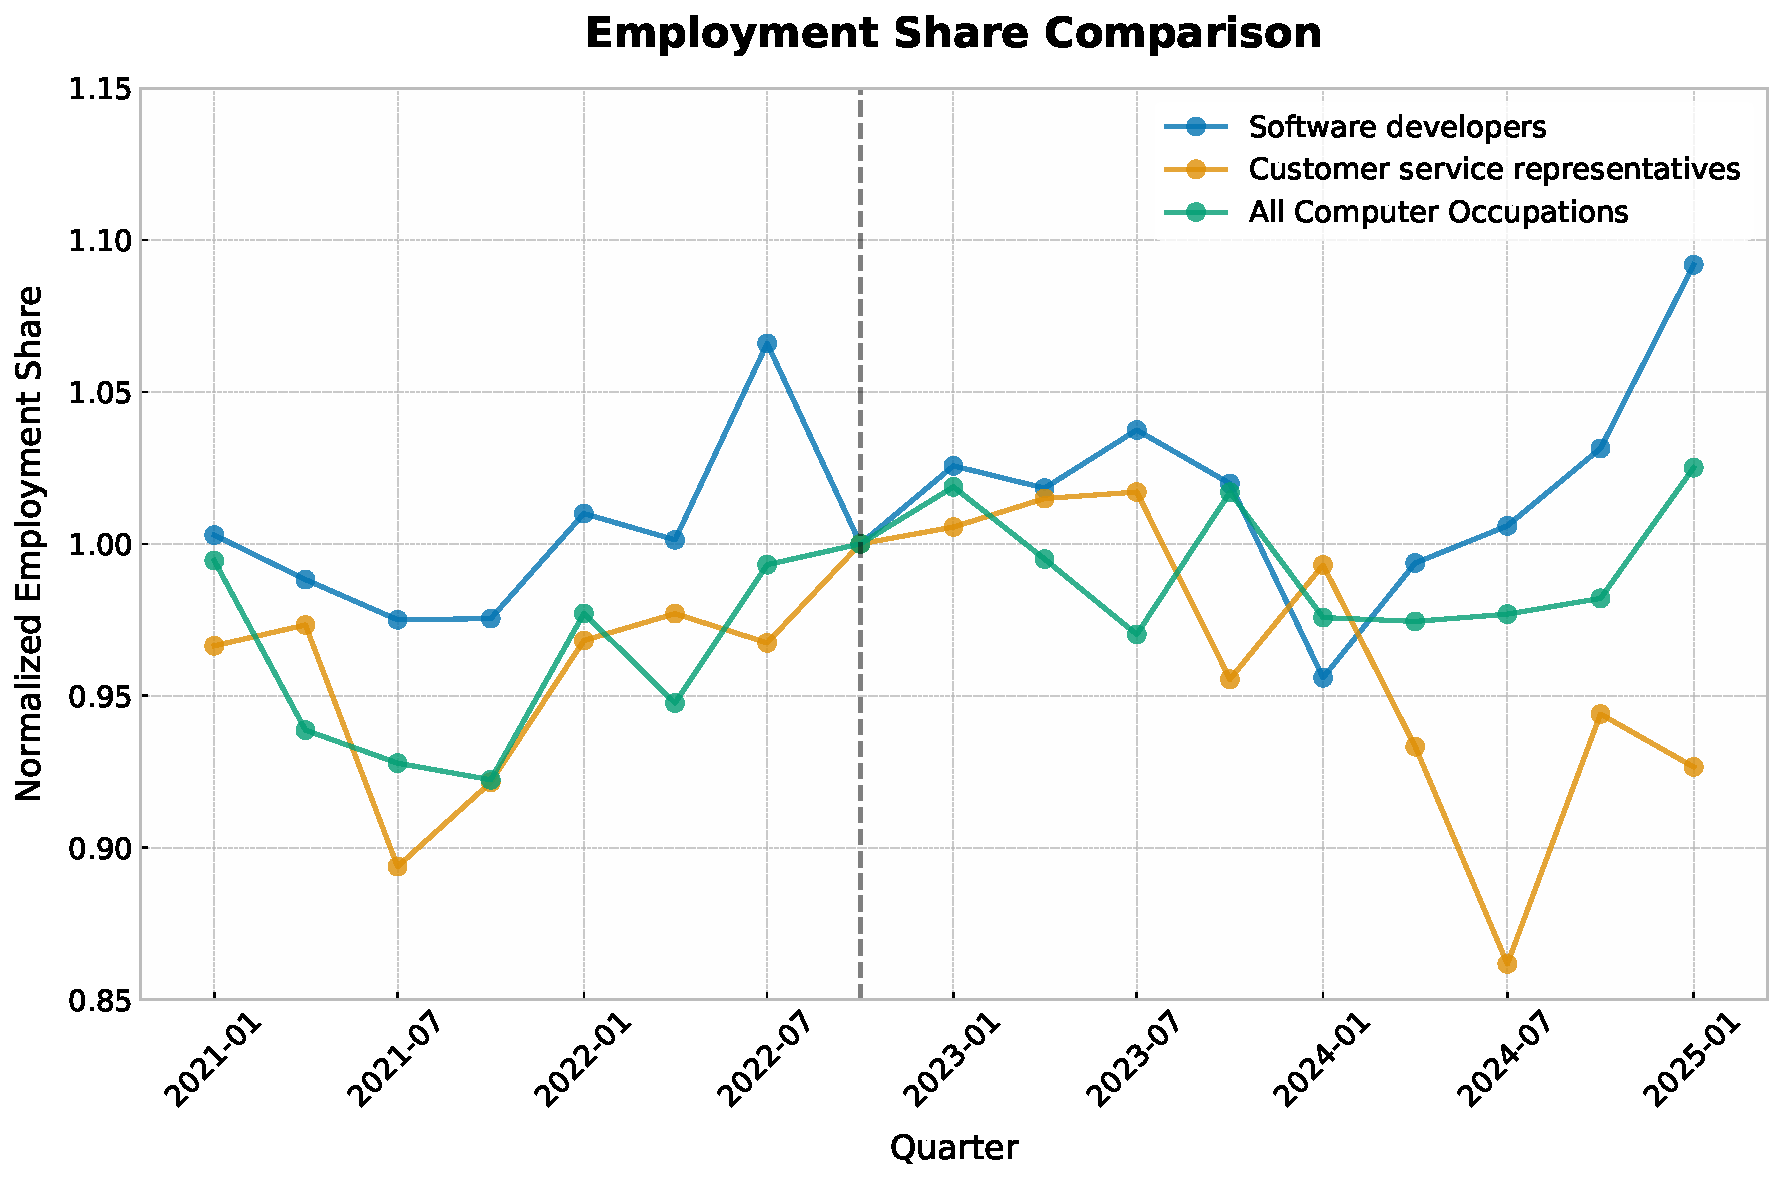
\includegraphics[width=0.8\textwidth]{../figures/employment_share_comparison_2021Q1.pdf}
  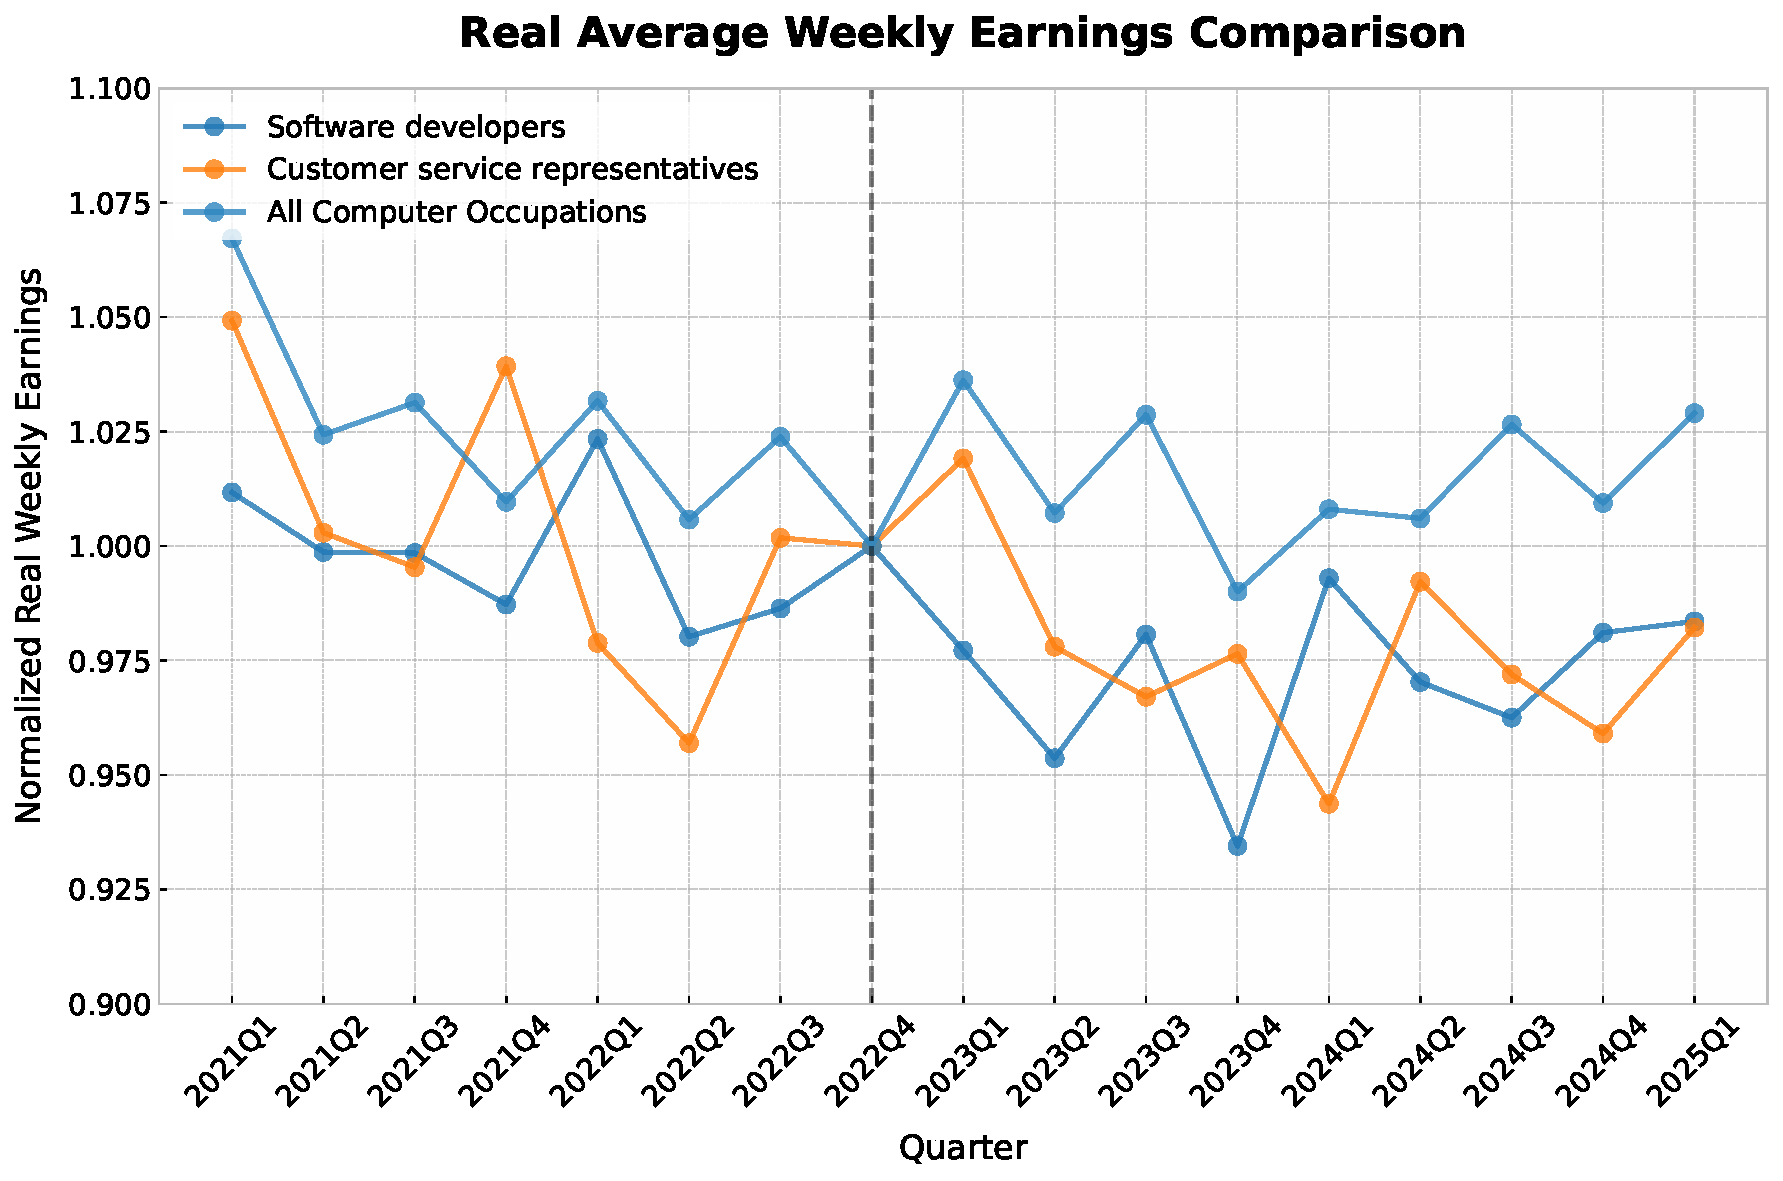
\includegraphics[width=0.8\textwidth]{../figures/earnings_comparison_combined_2021Q1.pdf}
	\caption{Employment share and real earnings trends for software developers, computer occupations, and customer service representatives. Computer occupations include all occupations with Census occupation codes 1005 through 1108.}
	\label{fig:employment_share_comparison_2021Q1}
\end{figure}



These findings raise the question of which occupational characteristics may influence the employment effects of AI given some level of measured exposure. Figure \ref{fig:employment_share_change_by_education_2022q4} shows employment trends for the most exposed quartile of occupations split by whether the college share in the occupation is above or below the median. The results suggest employment share increases in more educated exposed occupations and employment share declines in less educated exposed occupations in the periods before and after the release of ChatGPT. 

\begin{figure}[htbp]
	\centering
  \includegraphics[width=0.8\textwidth]{../figures/employment_share_change_by_education_2021q1.pdf}
  \includegraphics[width=0.8\textwidth]{../figures/real_earnings_change_by_education_2021q1.pdf}
	\caption{Employment share and real earnings trends for the most exposed quartile of occupations, split by whether the occupation has above medican or below median college share. }
	\label{fig:employment_share_change_by_education_2022q4}
\end{figure}


\subsection{Labor Market Trends for Entry-Level Workers}

In recent months there has been a growing concern that AI is beginning to displace entry-level workers \citep{thompson_something_2025,raman_opinion_2025,allen_behind_2025}. The top panel of Figure  \ref{fig:employment_share_entry_level_overall} shows the employment share trends for entry level versus experienced workers. The analysis shows that entry level workers have cyclical and volatile employment compared to more experienced workers, with no notable overall trend in employment shares over the sample period. The bottom panel likewise shows no evident trend in real earnings. 

\begin{figure}[htbp]
	\centering
  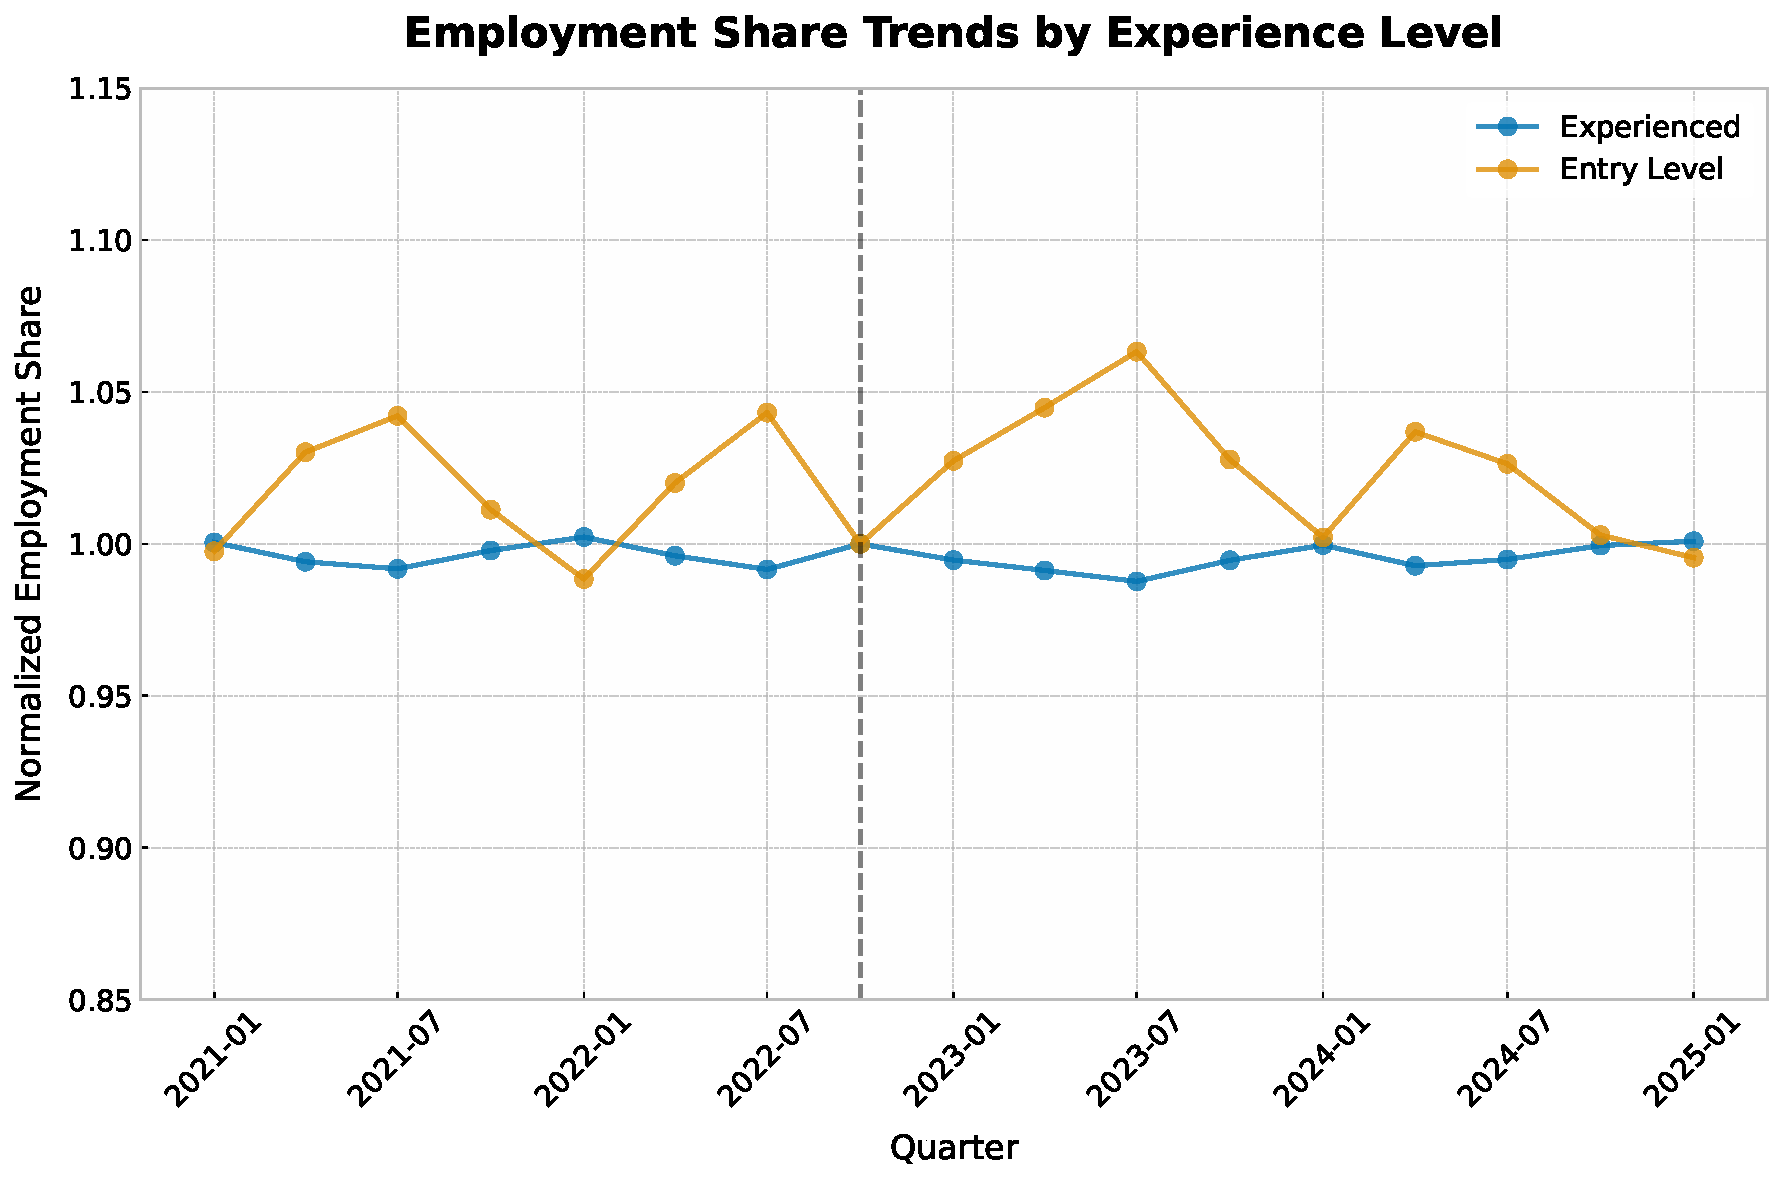
\includegraphics[width=0.8\textwidth]{../figures/employment_share_entry_level_overall.pdf}
  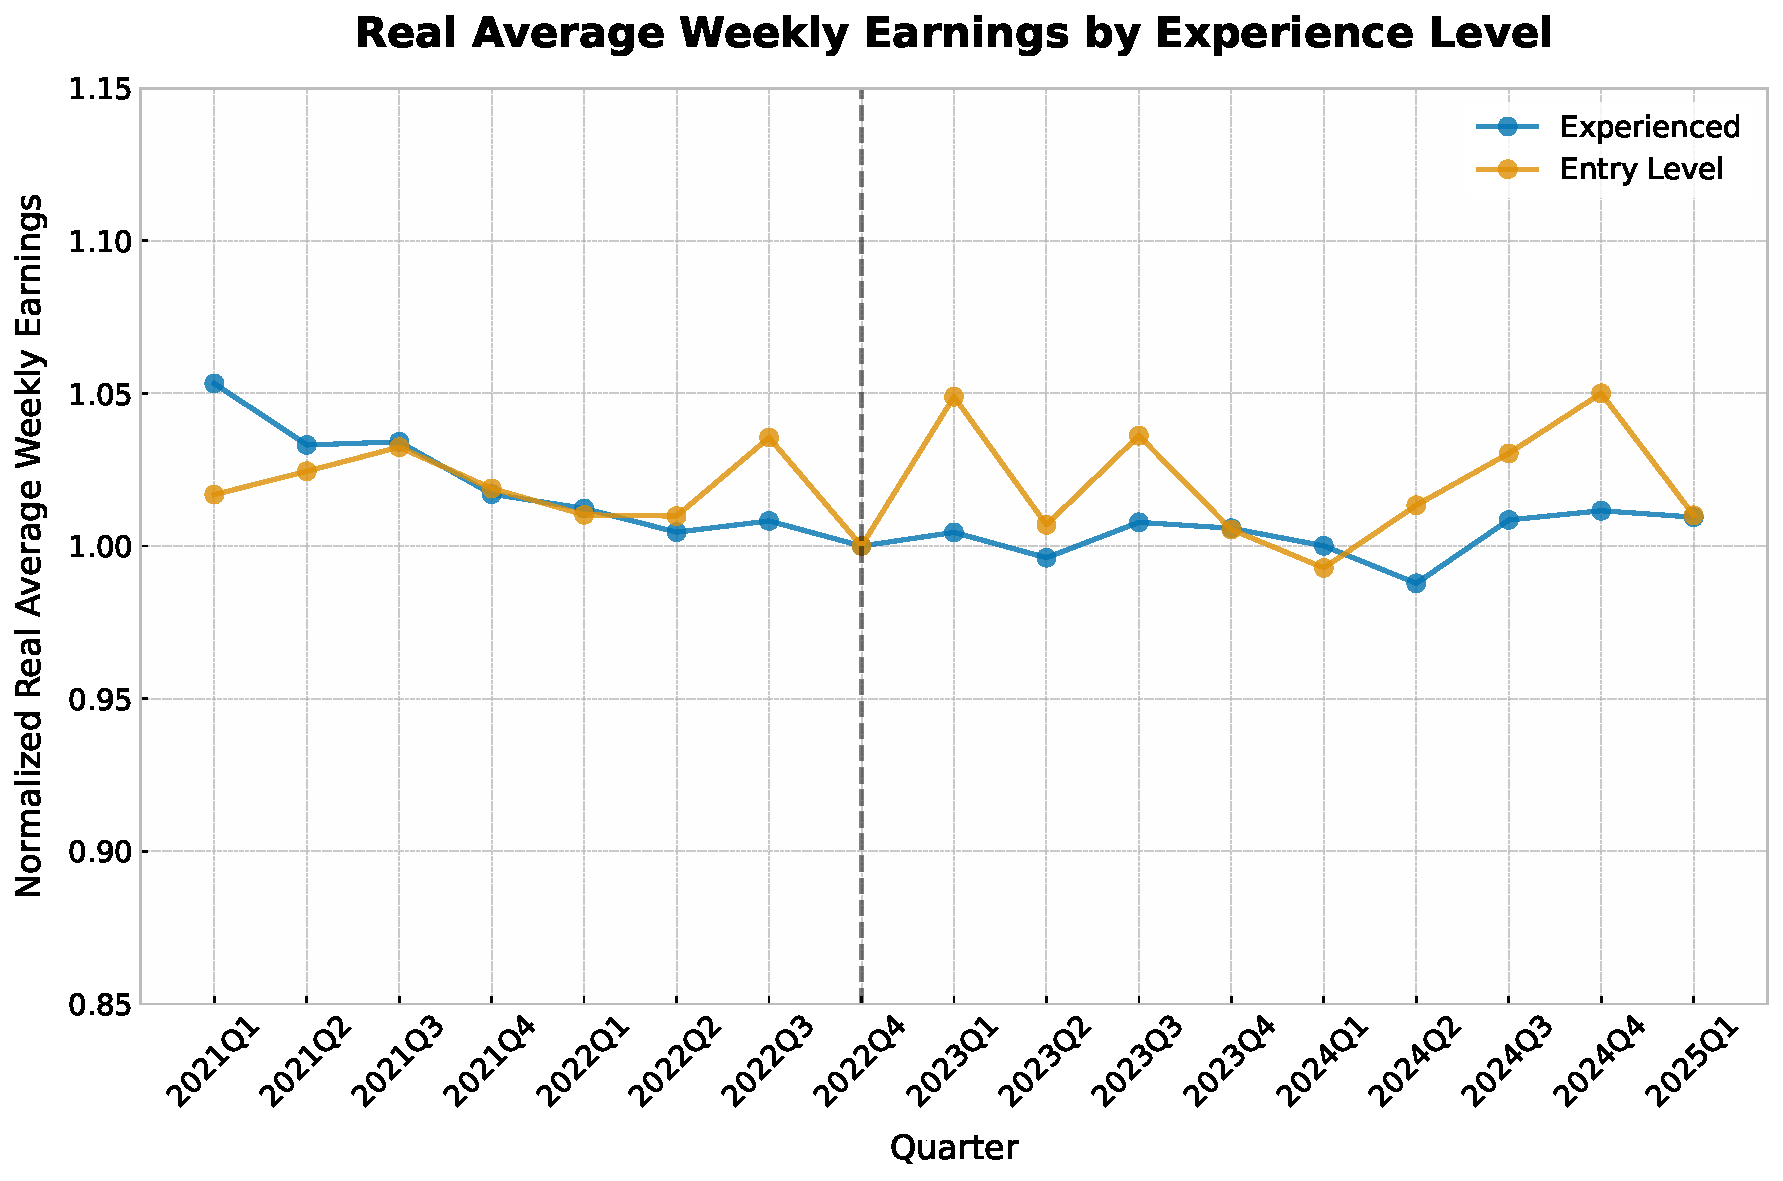
\includegraphics[width=0.8\textwidth]{../figures/real_earnings_by_entry_level.pdf}
	\caption{Employment share and real earnings trends for entry level versus experienced workers. Entry level workers are defined as workers aged 26 or younger. }
	\label{fig:employment_share_entry_level_overall}
\end{figure}

These patterns for entry level workers overall might mask trends in occupations more exposed to AI. Figure \ref{fig:employment_share_entry_level_2021Q1} shows the employment share trends for entry level versus experienced workers in the quartile of occupations most exposed to AI according to the GPT-4-based $\beta$ measure from \citet{eloundou_gpts_2024}. Figure \ref{fig:employment_share_entry_level_computer_occupations_2021Q1} similarly shows the employment trends for entry level versus experienced workers in computer occupations. Both plots are noisy, primarily because restricting to workers under the age of 26 reduces the sample size. With more time and larger surveys it may become apparent whether trends are sustained. 



\section{Relationship between Job Postings and Employment}

The general purpose nature of artificial intelligence has raised concerns of widespread employment declines, with some speculation that these trends are already visible within certain industries such as software development. One piece of evidence taken to suggest employment declines already are in job posting trends from sources such as Indeed. As shown in Figure \ref{fig:job_postings_by_sector}, the number of job postings for software developers has fallen since a peak in early 2022. 

Three aspects of the data suggest caution in interpreting the job posting trends to signal labor market disruption for software developers caused by AI. 
\begin{enumerate}
	\item The number of job postings has fallen for a range of other occupations as well, including in professions such as nursing with low estimated AI exposure. This suggests that the decline is not specific to software developers. 
	\item While the decline is steeper for software developers than other professions, the peak in early 2022 is also considerably higher. This could indicate macroeconomic trends in the tech sector that led to a boom and bust in job postings unrelated to AI. 
	\item The decline in job postings is not matched by a decline in employment in the software development occupation in the CPS, as shown in Figure \ref{fig:employment_share_comparison_2021Q1}. If anything there is some evidence of an increase in employment in software development. These findings suggest that job posting and employment trends need not coincide and may offer different, complementary signals for tracking trends in the job market. Another way to see this is that the trend in Figure \ref{fig:job_postings_by_sector} occurred across sectors even as the US national unemployment rate and labor force participation rate remained relatively stable. 
\end{enumerate}



What explains the divergence between job posting trends and employment trends? Growing labor demand would explain employment growth for software developers but not declines in job postings. Growing labor supply would also explain greater employment for software developers but not stable wages, all else equal. Explaining these trends requires a more nuanced story that would be valuable to explore in future work.\footnote{Another explanation is that a smaller share of jobs are posted on Indeed, though sites such as Ashby and TrueUp find similar patterns \citep{Codell2023_TrendsReport, Rachitsky2025_ProductMarket}.} 

\begin{figure}[htbp]
	\centering
  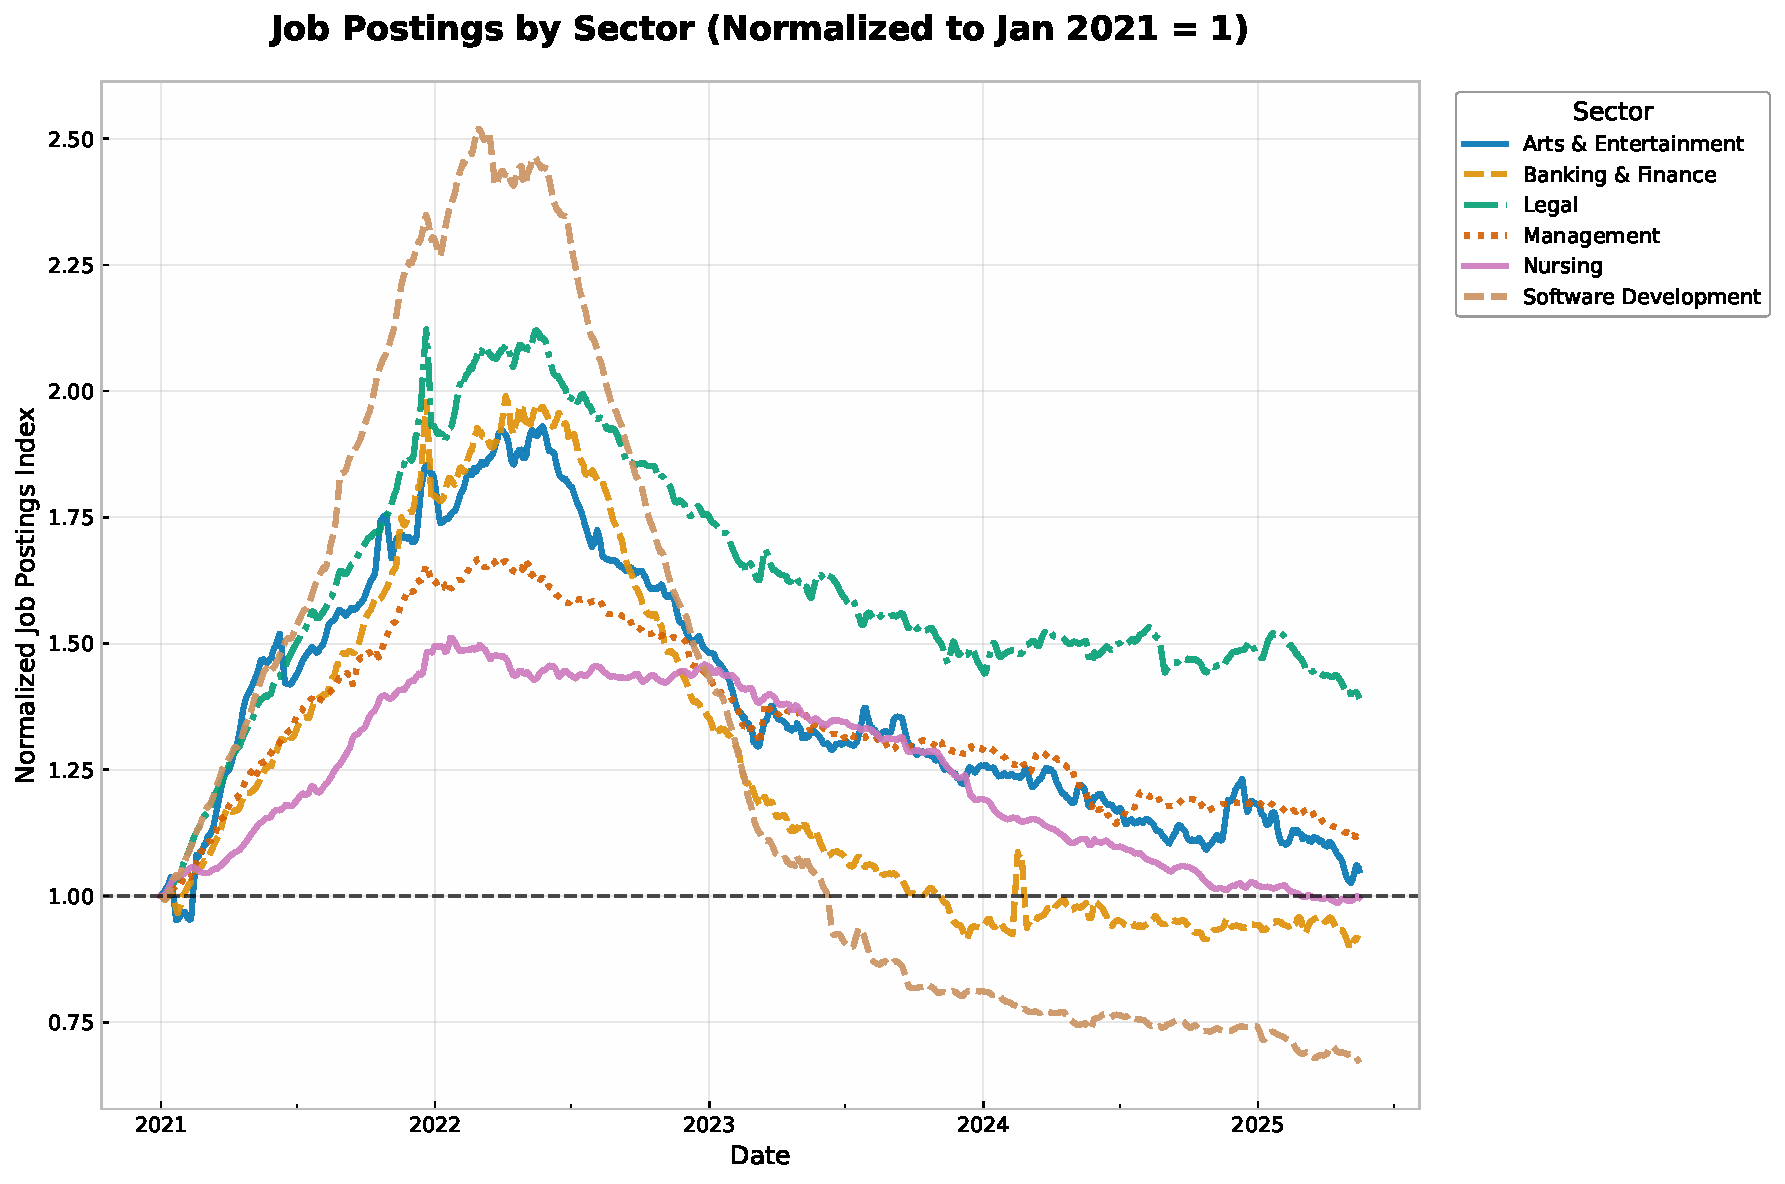
\includegraphics[width=.95\textwidth]{../figures/job_postings_by_sector.pdf}
	\caption{Job postings trends for software developers and other occupations. Data comes from Indeed.}
	\label{fig:job_postings_by_sector}
\end{figure}

\section{Conclusion}

This paper uses the CPS to provide an empirical snapshot of the US labor market in the initial years since the generative AI revolution. Overall, occupations highly exposed to AI have not experienced employment declines. However, within this group, employment in occupations like software development continues to grow, while it has fallen in like customer service. These trends are correlated with occupational education levels. 

These results for employment and earnings contrast with trends in job posting data. This divergence serves as a methodological caution for using job postings as a proxy for these other labor market indicators.

Further research that provides real-time tracking of employment in AI-exposed occupations using large-scale administrative or survey data would be invaluable for assessing how these new technologies are shaping the labor market. 






\bibliographystyle{ecta}
\bibliography{../../../bibliography}

\clearpage


\appendix

\setcounter{figure}{0}
\renewcommand{\thefigure}{A\arabic{figure}}
\setcounter{table}{0}
\renewcommand{\thetable}{A\arabic{table}}

\section*{\centering{\textsc
{Appendix}}\\[0.6cm]
}

\begin{figure}[htbp]
	\centering
  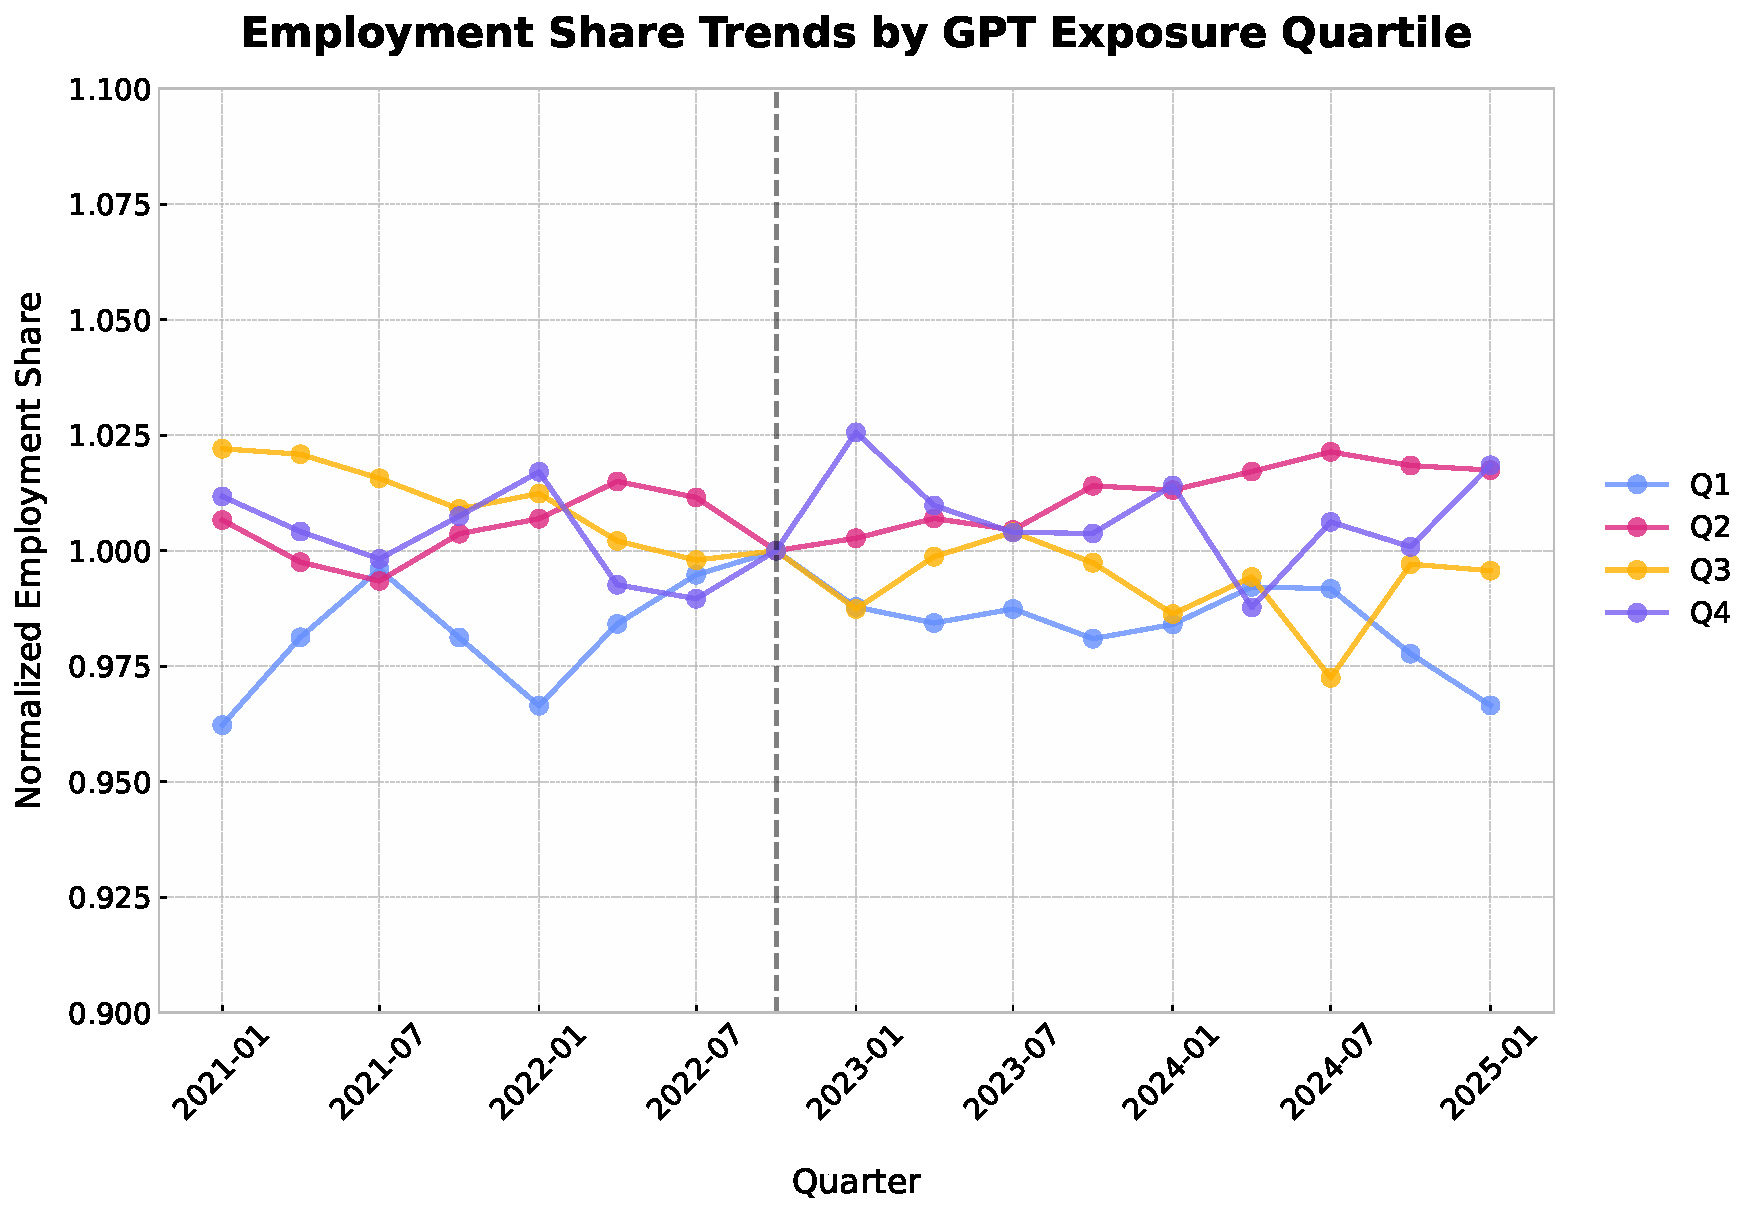
\includegraphics[width=0.8\textwidth]{../figures/employment_share_by_gpt4_alpha_quartile_2021Q1.pdf}
  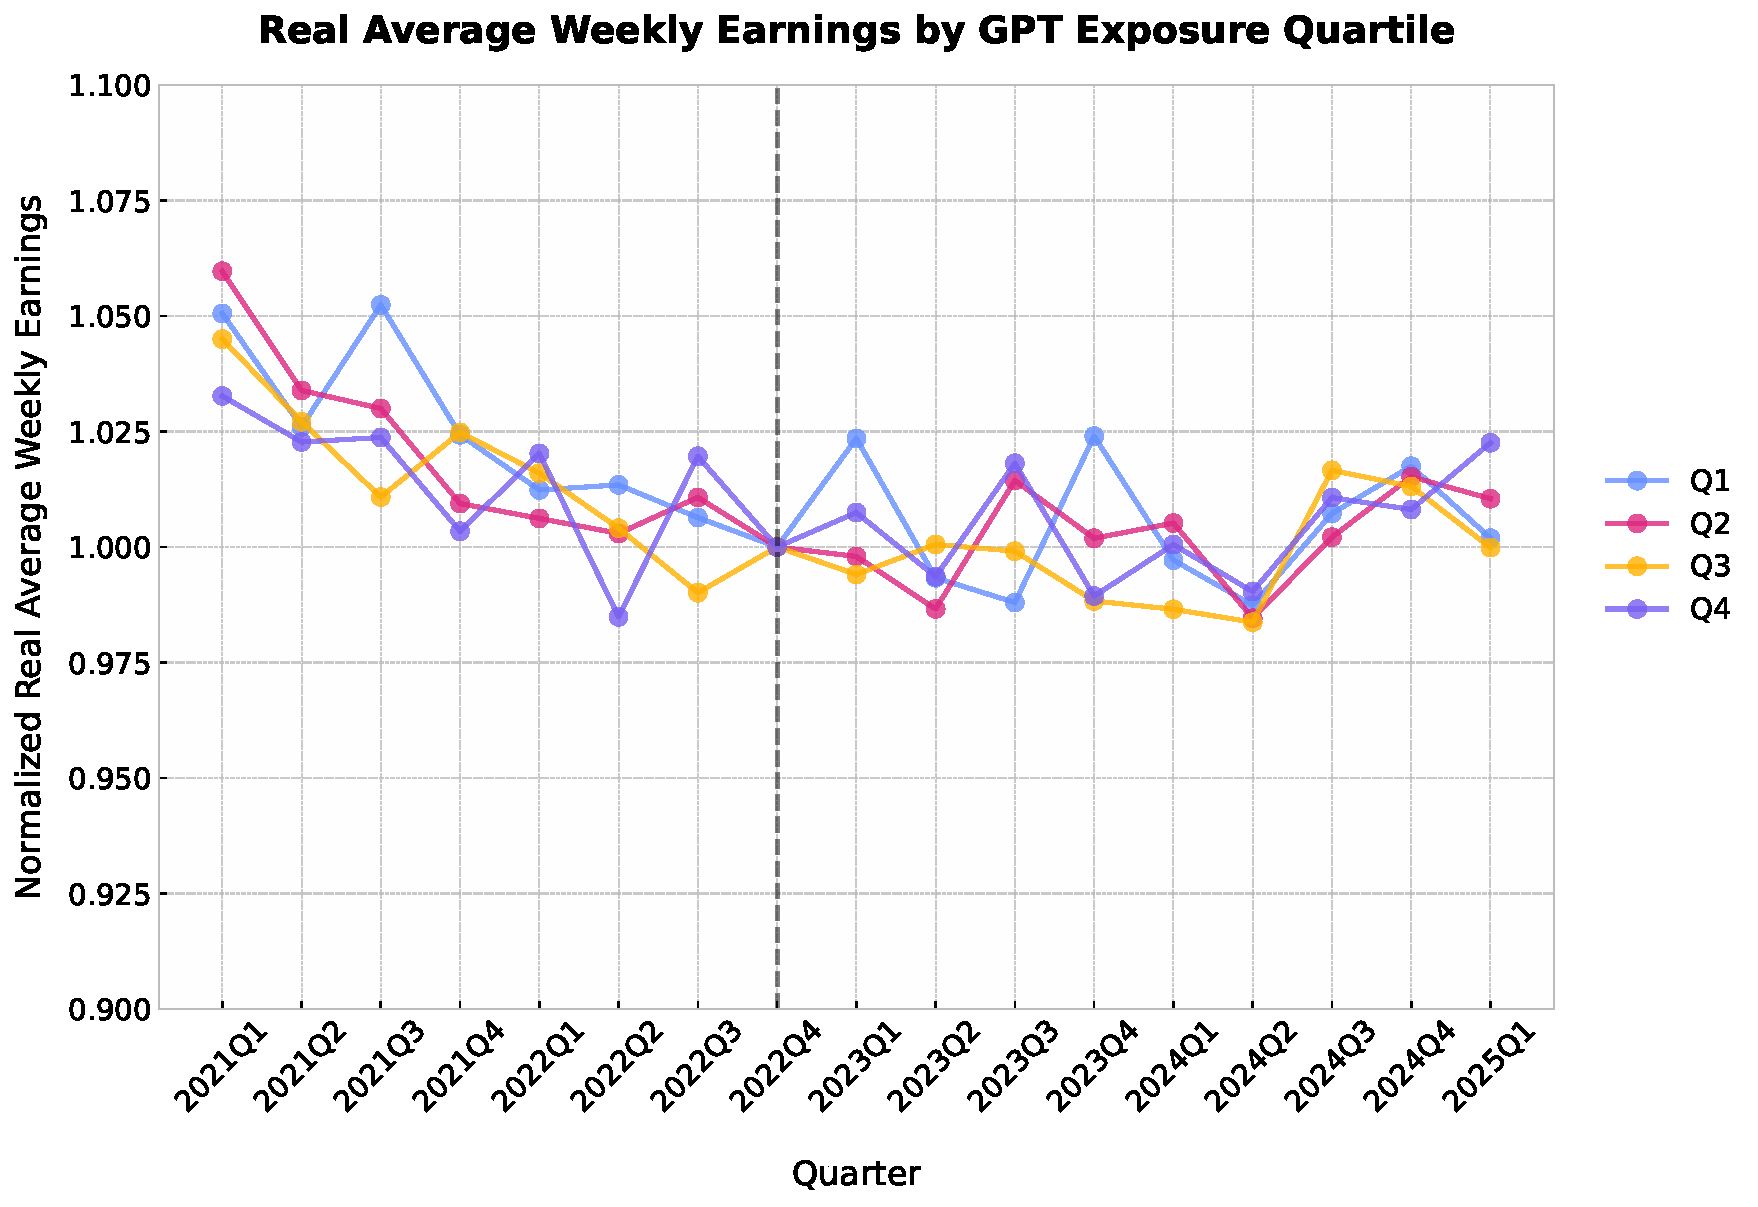
\includegraphics[width=0.8\textwidth]{../figures/real_earnings_by_gpt4_alpha_quartile_2021Q1.pdf}
	\caption{Employment share and real earnings trends by AI exposure using the GPT-4-based $\alpha$ measure from \citet{eloundou_gpts_2024}.}
	\label{fig:employment_trends_alpha}
\end{figure}

\begin{figure}[htbp]
	\centering
  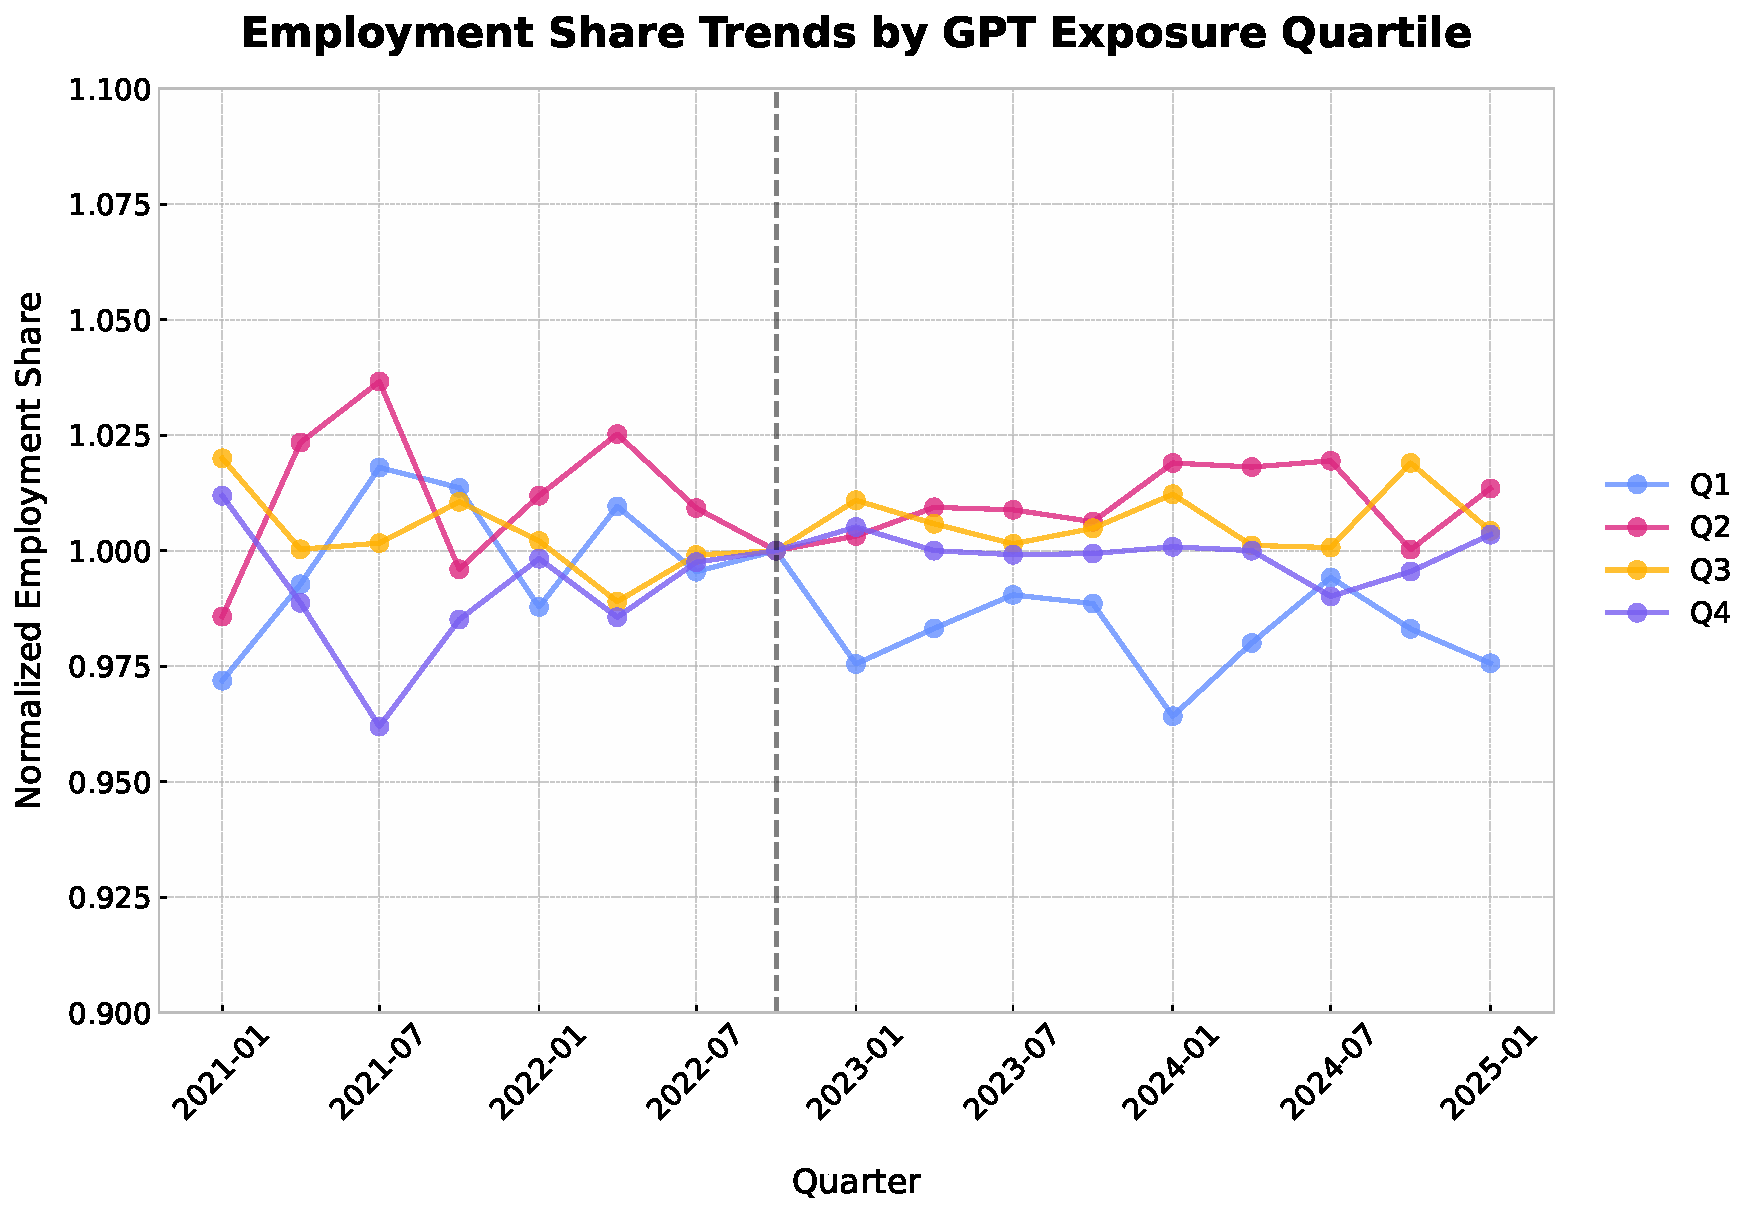
\includegraphics[width=0.8\textwidth]{../figures/employment_share_by_gpt4_gamma_quartile_2021Q1.pdf}
  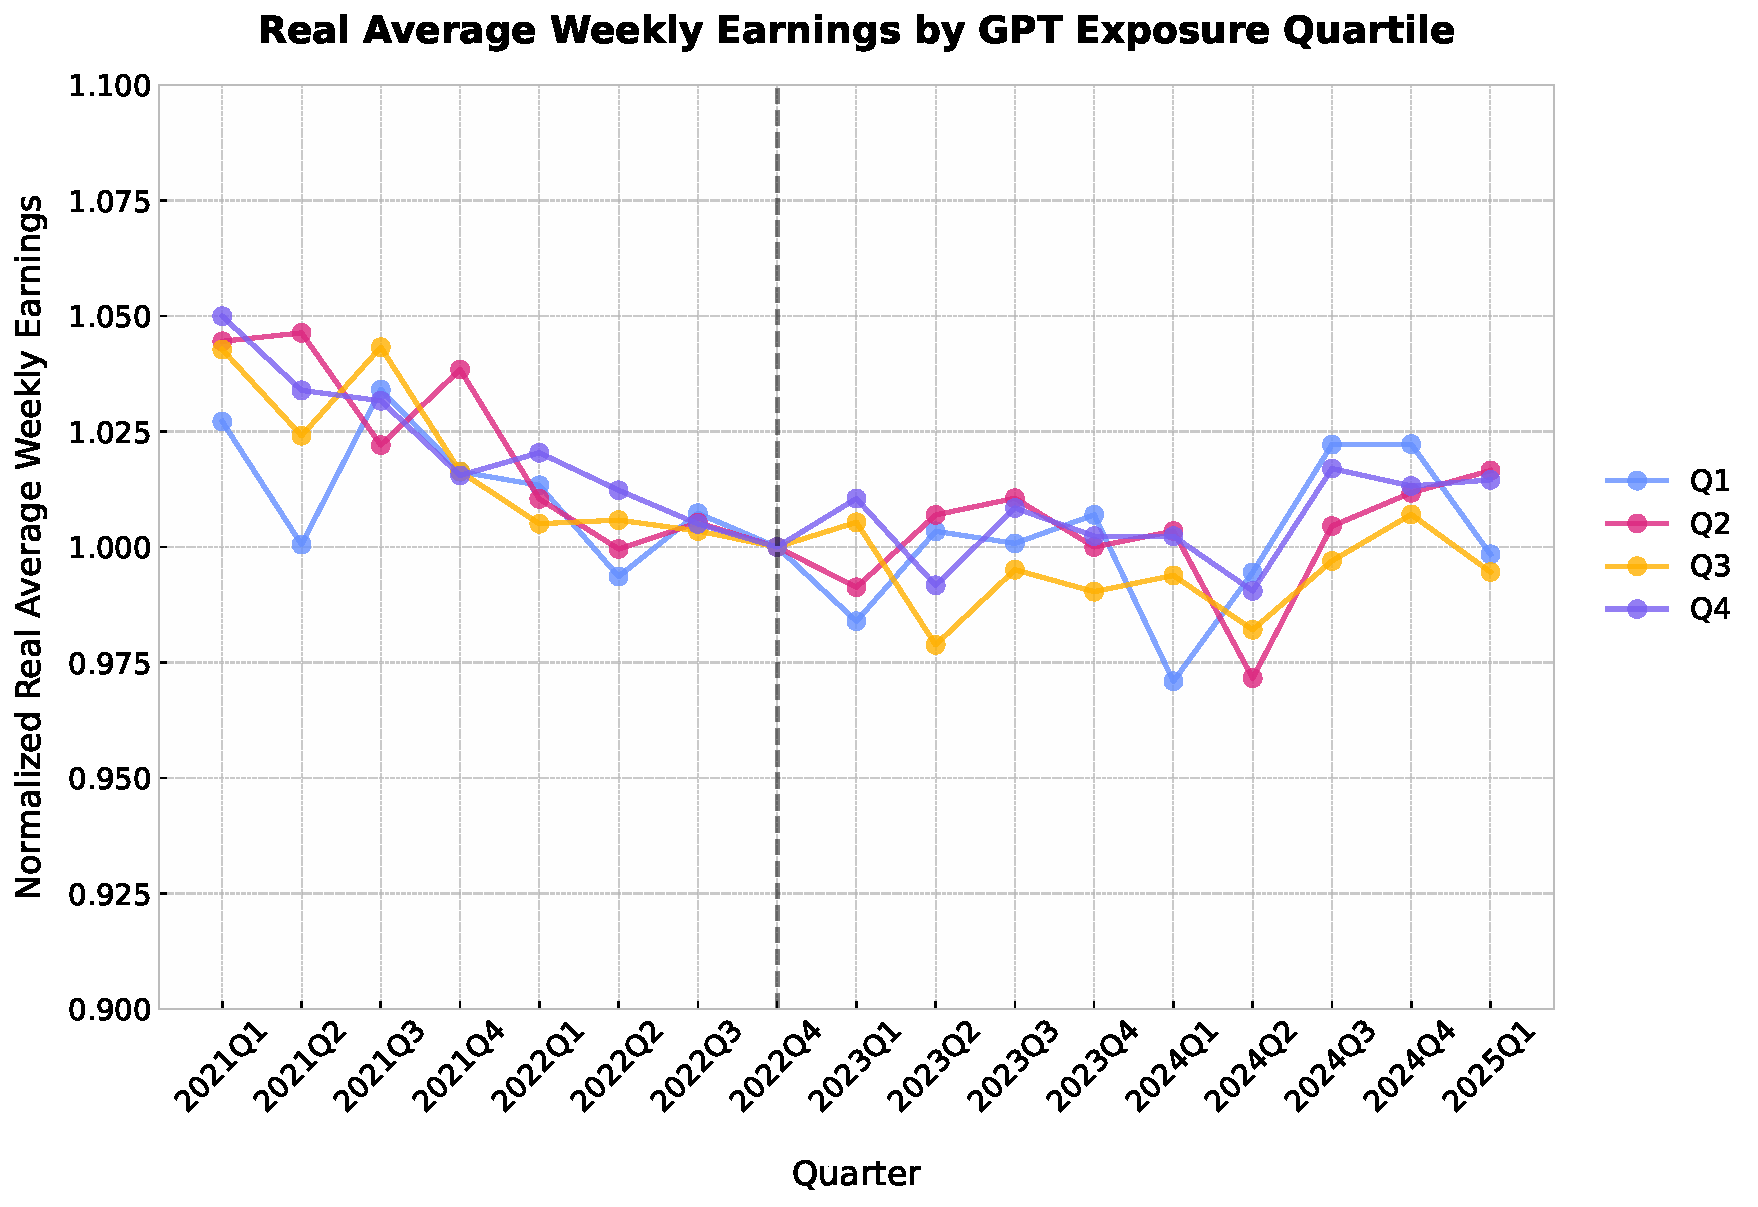
\includegraphics[width=0.8\textwidth]{../figures/real_earnings_by_gpt4_gamma_quartile_2021Q1.pdf}
	\caption{Employment share and real earnings trends by AI exposure using the GPT-4-based $\gamma$ measure from \citet{eloundou_gpts_2024}.}
	\label{fig:employment_trends_gamma}
\end{figure}

\begin{figure}[htbp]
	\centering
  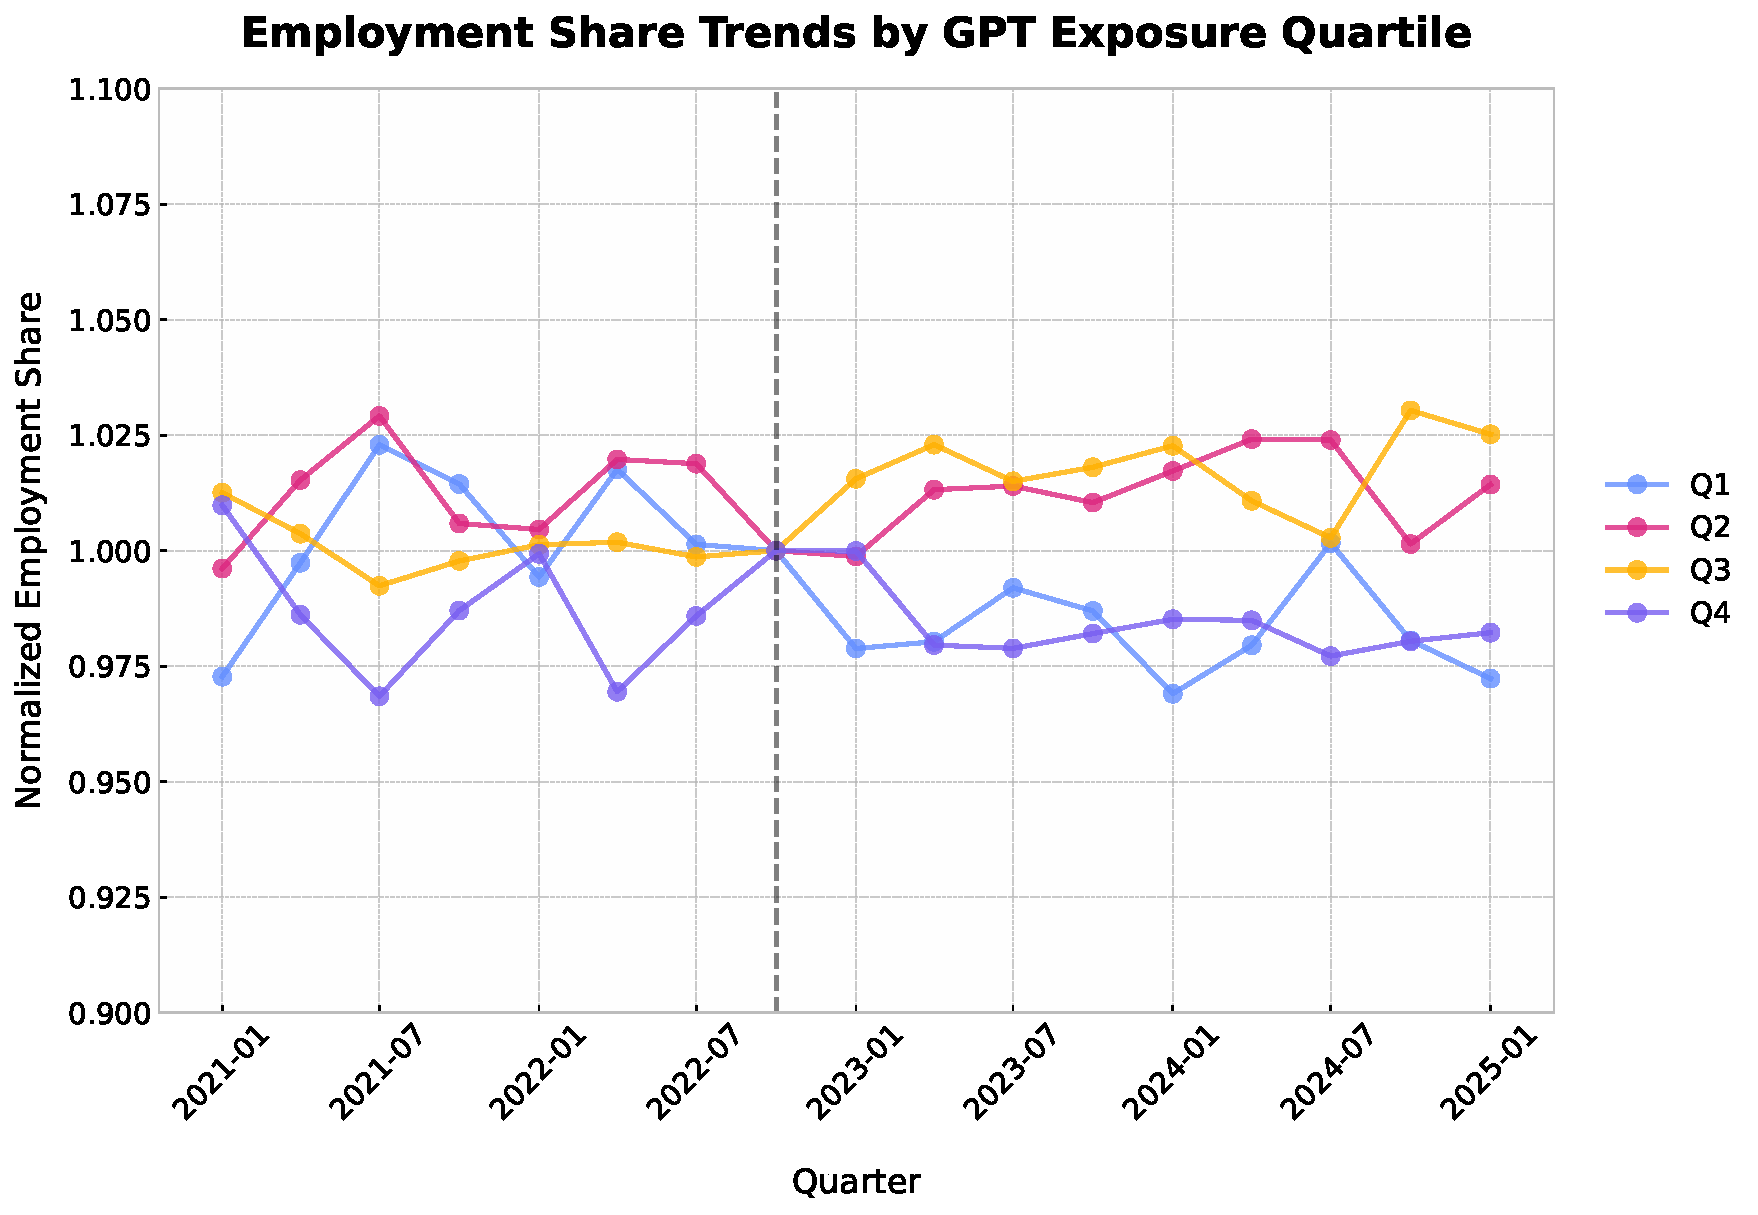
\includegraphics[width=0.8\textwidth]{../figures/employment_share_by_automation_quartile_2021Q1.pdf}
  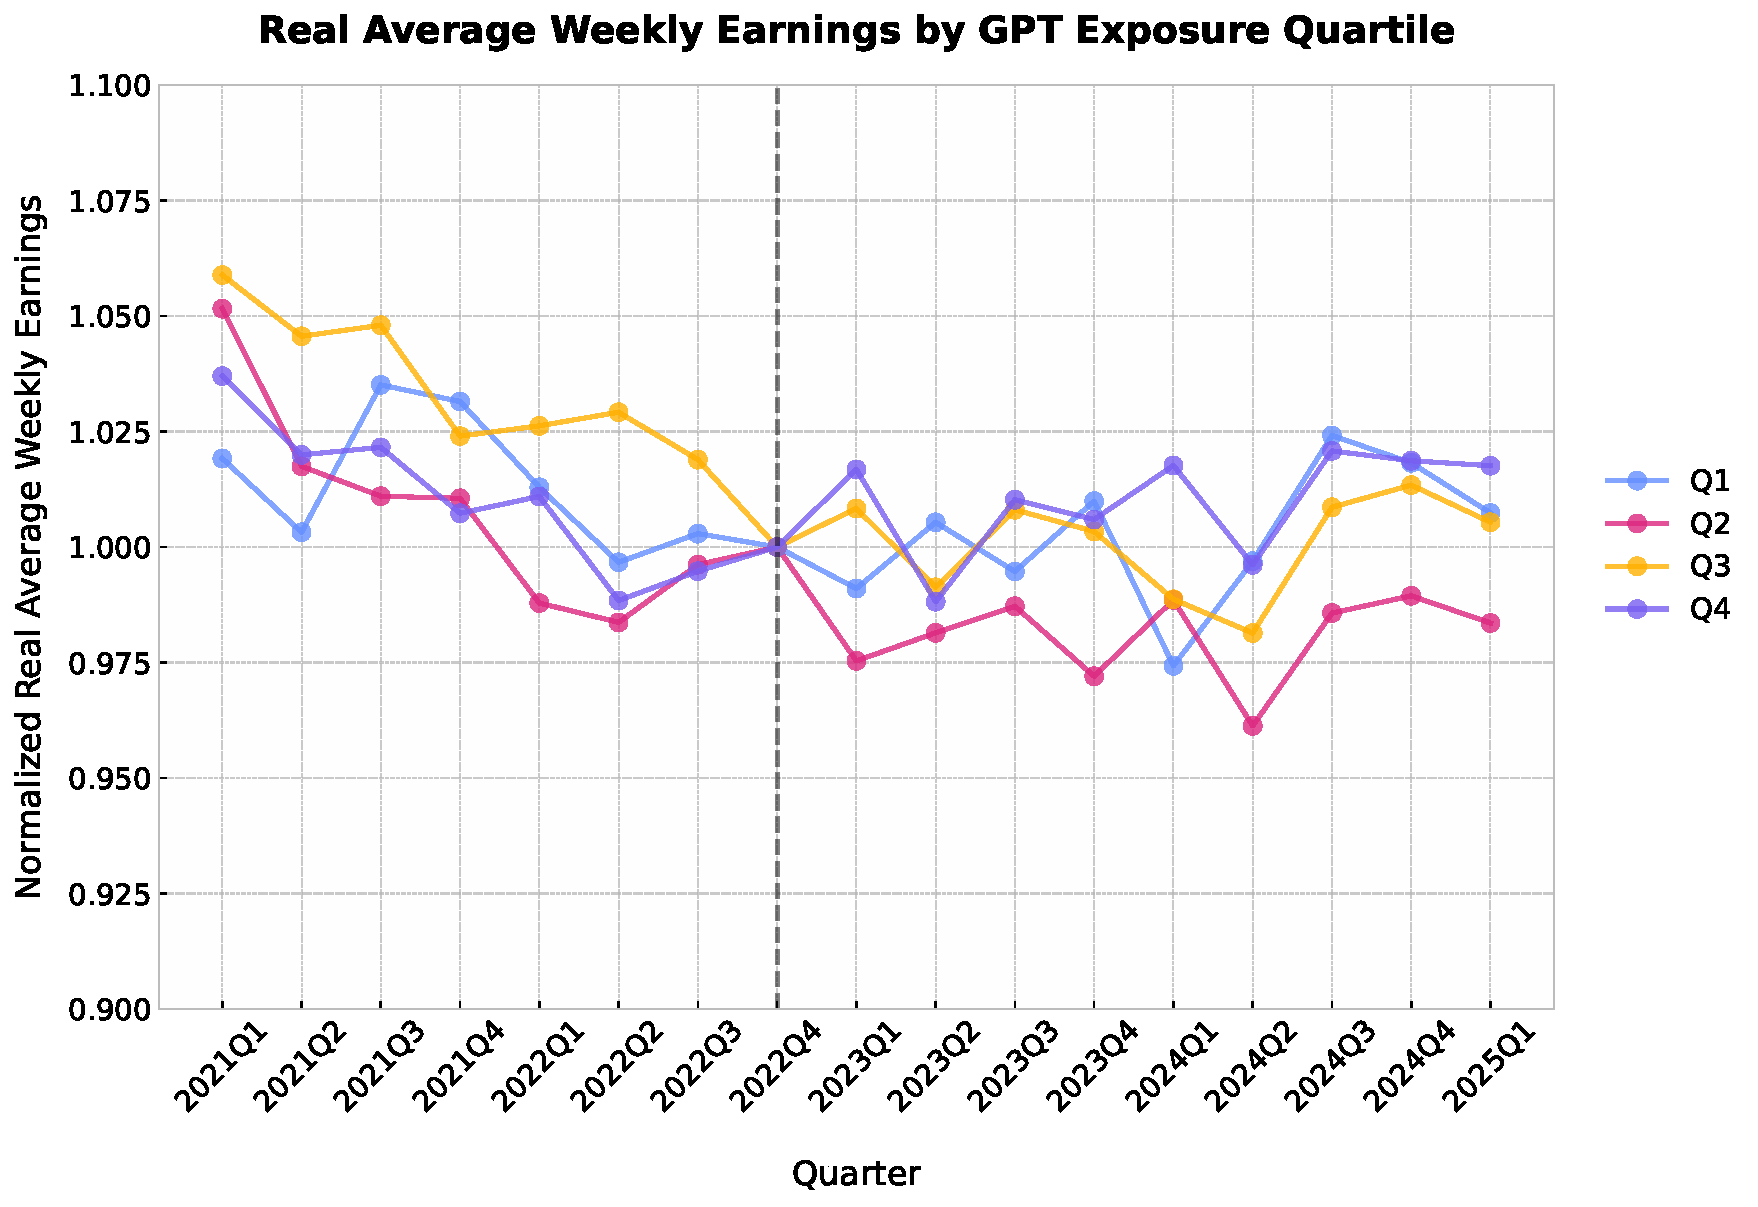
\includegraphics[width=0.8\textwidth]{../figures/real_earnings_by_automation_quartile_2021Q1.pdf}
	\caption{Employment share and real earnings trends by AI exposure using the GPT-4-based automation measure from \citet{eloundou_gpts_2024}.}
	\label{fig:employment_trends_automation}
\end{figure}




\begin{figure}[htbp]
	\centering
  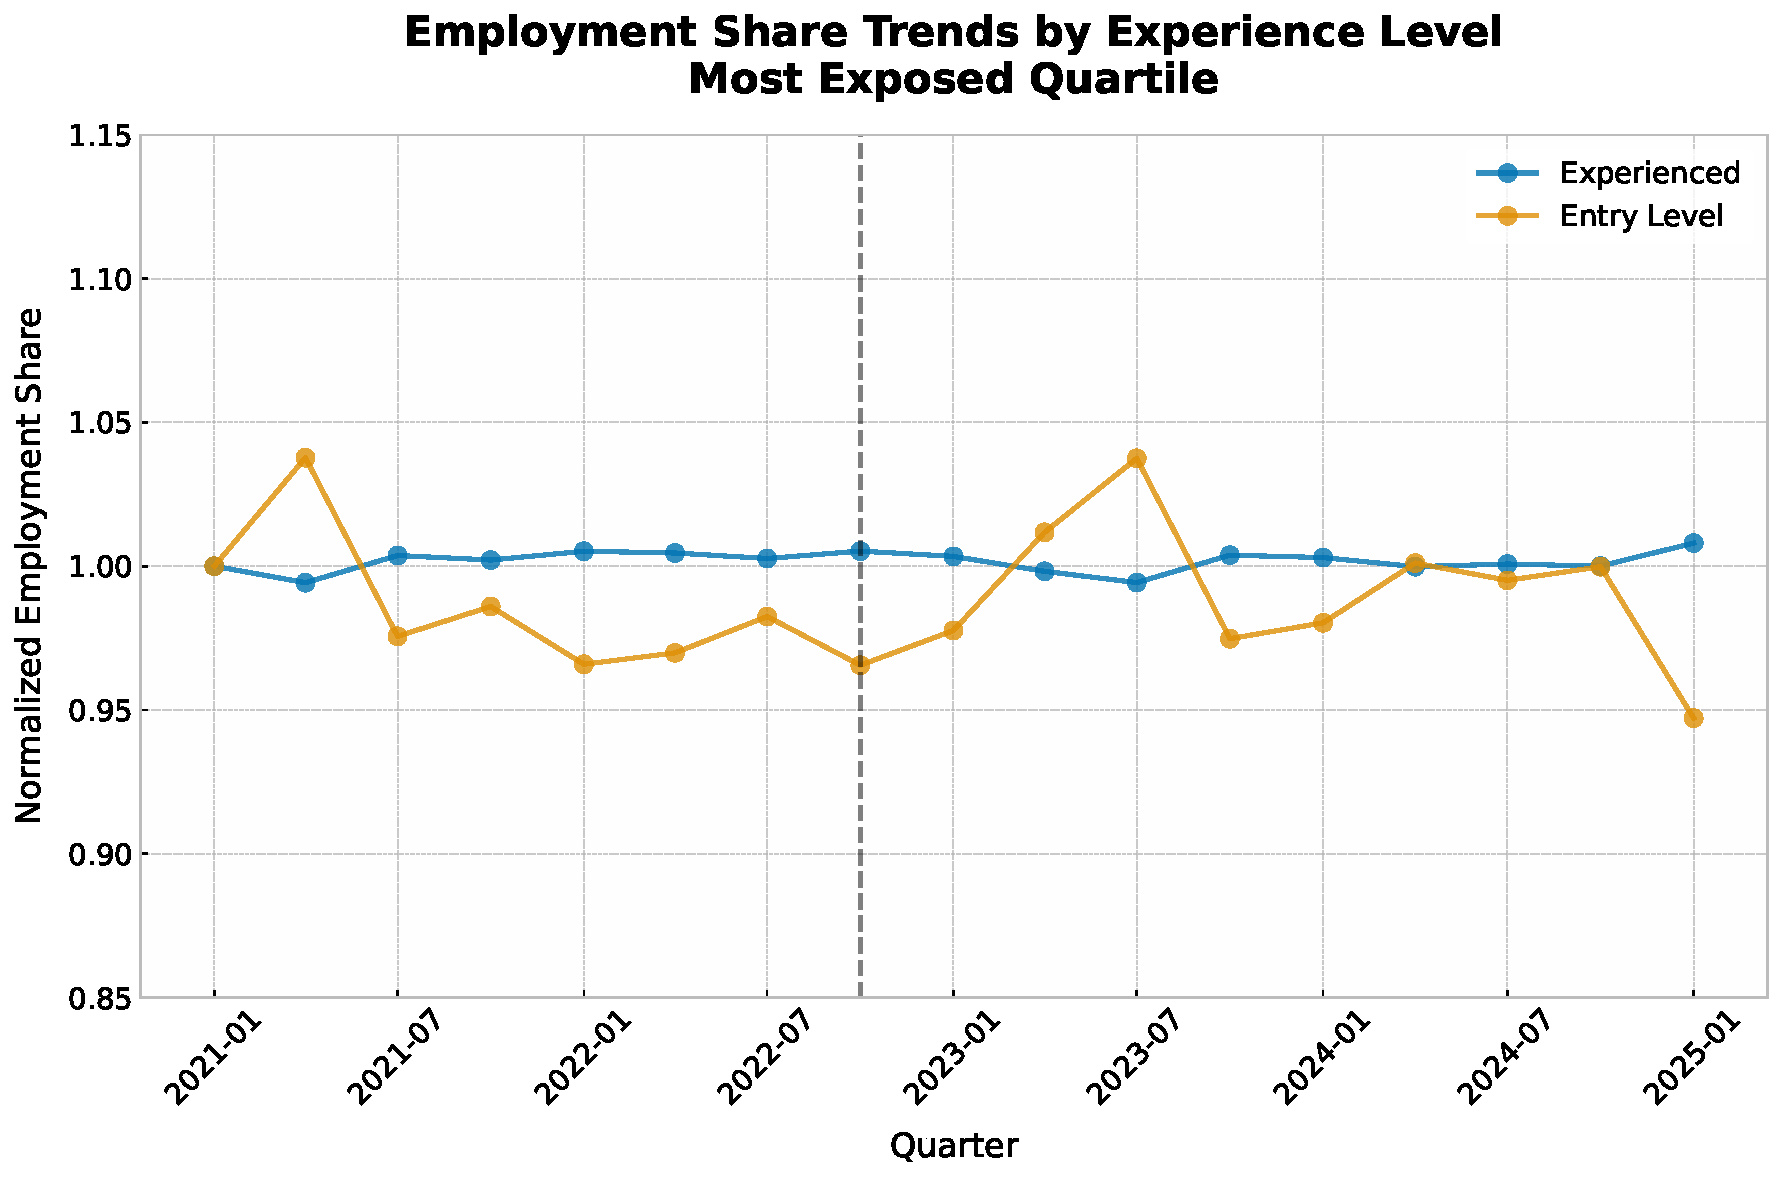
\includegraphics[width=0.8\textwidth]{../figures/employment_share_entry_level_2021Q1.pdf}
  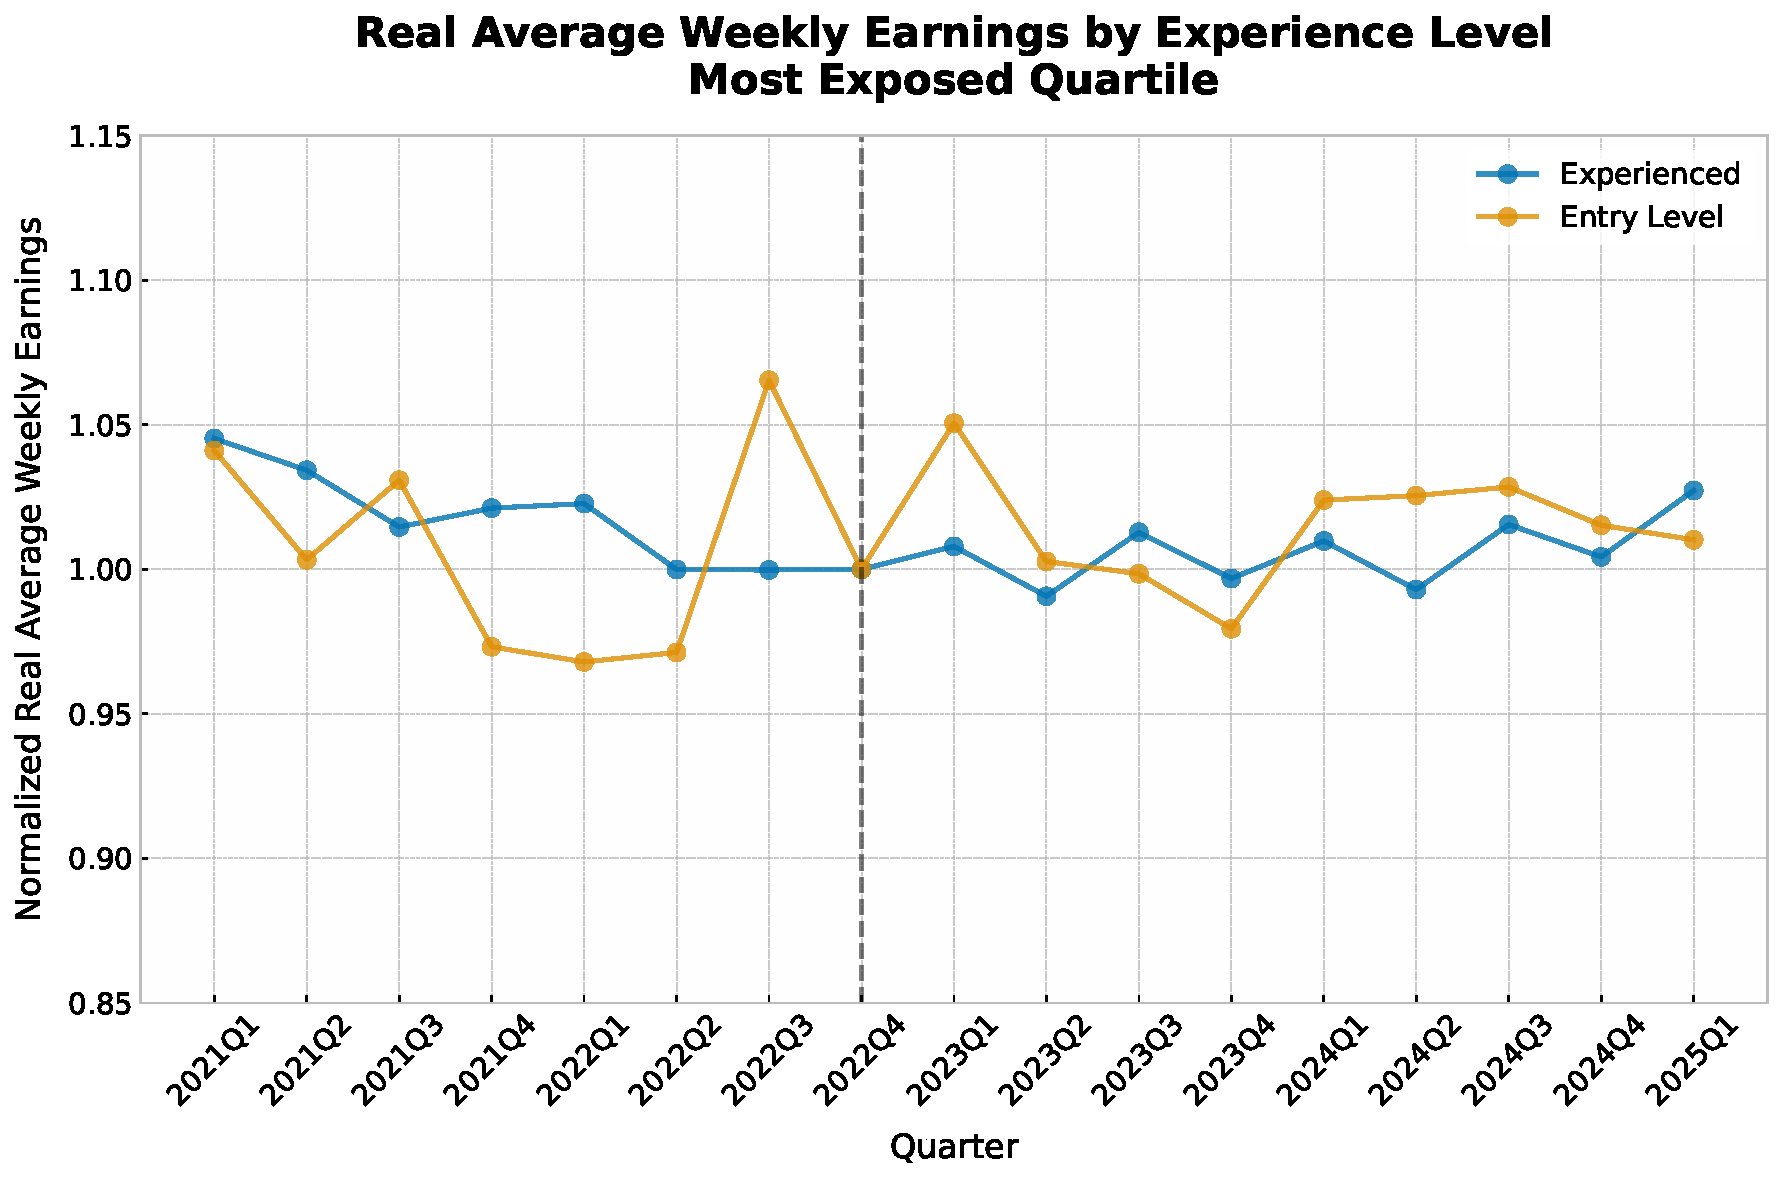
\includegraphics[width=0.8\textwidth]{../figures/real_earnings_by_entry_level_exposed.pdf}
	\caption{Employment share and real earnings trends for entry level versus experienced workers, restricted to the most AI-exposed quartile of occupations. Entry level workers are defined as workers aged 26 or younger. }
	\label{fig:employment_share_entry_level_2021Q1}
\end{figure}


\begin{figure}[htbp]
	\centering
  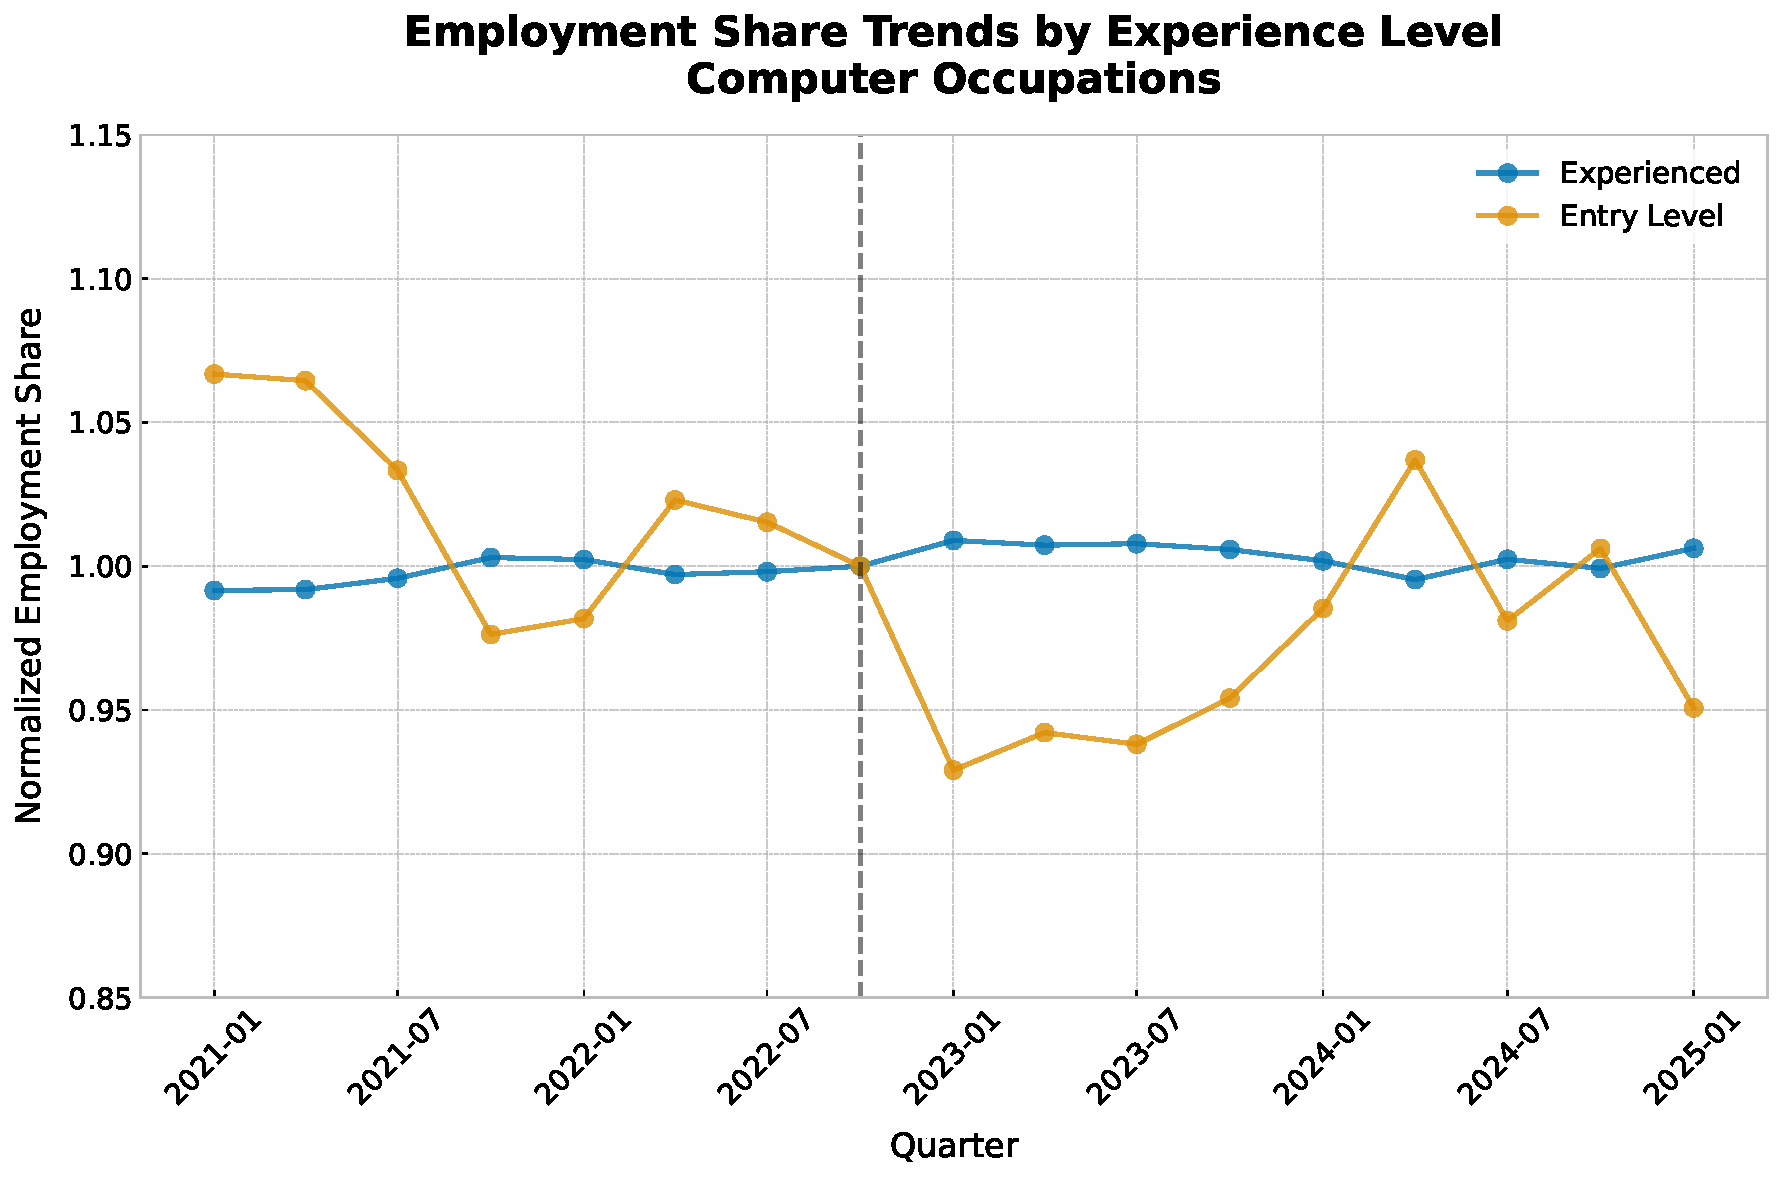
\includegraphics[width=0.8\textwidth]{../figures/employment_share_entry_level_computer_occupations_2021Q1.pdf}
  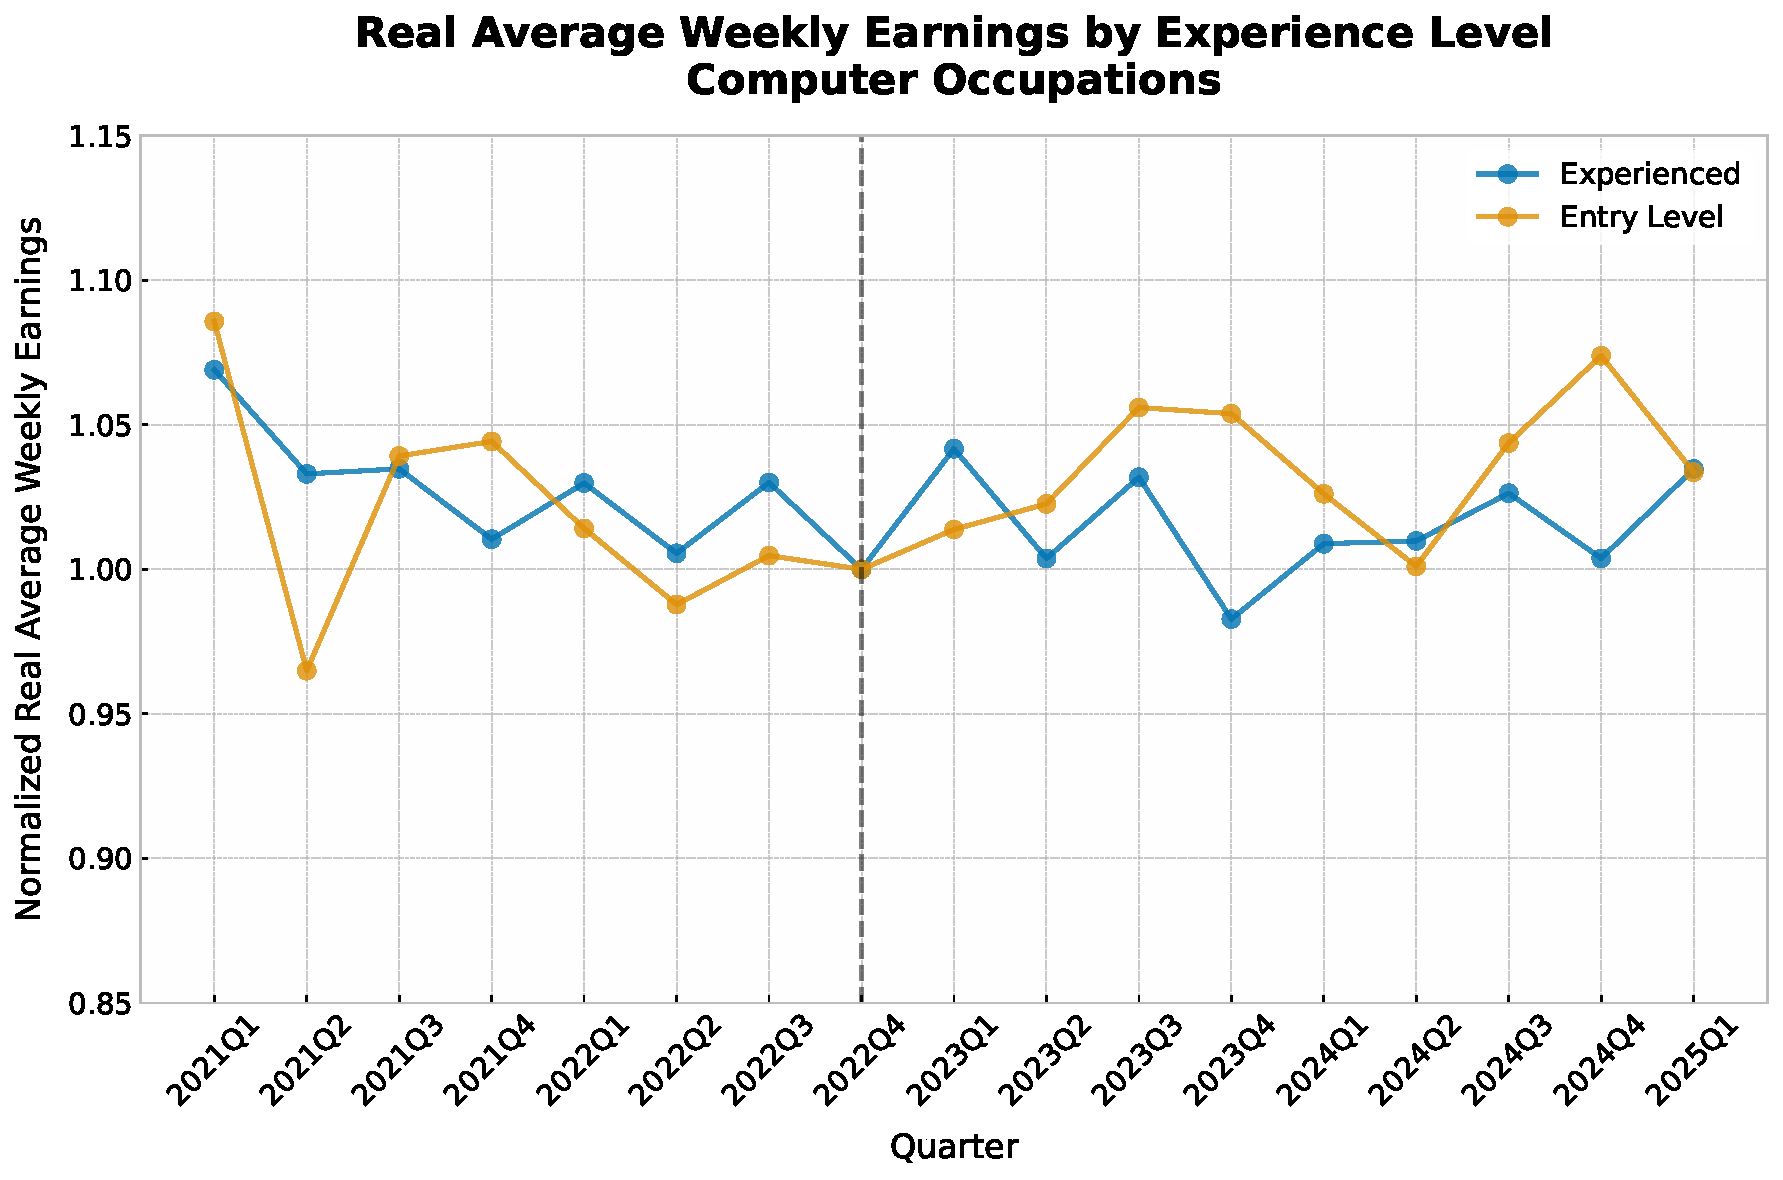
\includegraphics[width=0.8\textwidth]{../figures/real_earnings_by_entry_level_computer.pdf}
	\caption{Employment share and real earnings trends for entry level versus experienced workers, restricted to the most computer occupations corresponding to Census occupation codes 1005 through 1108. Entry level workers are defined as workers aged 26 or younger. }
	\label{fig:employment_share_entry_level_computer_occupations_2021Q1}
\end{figure}





\end{document}
